\documentclass[openany]{scrreprt}
\usepackage[utf8]{inputenc}

% quotes
\usepackage{csquotes}
\usepackage{tcolorbox}
\usepackage{listings}
%\usepackage{underscore}
\usepackage[hyphens,spaces,obeyspaces]{url}
\usepackage[bookmarks=true]{hyperref}
\usepackage[english]{babel}
\usepackage{booktabs}
\usepackage{graphicx}
\usepackage{longtable}
\usepackage{float}
\usepackage{mdframed}
\usepackage[htt]{hyphenat}

\newmdenv[
  topline=true,
  bottomline=true,
  skipabove=\topsep,
  skipbelow=\topsep
]{siderules}

\newtcolorbox{textbox}[1][]{
	standard jigsaw,
	opacityback=0
}

\lstset{
  basicstyle=\ttfamily,
  columns=fullflexible,
  frame=single,
  breaklines=true,
  postbreak=\mbox{\textcolor{red}{$\hookrightarrow$}\space},
}

\hypersetup{
pdftitle={Spring Boot},			% title
pdfauthor={Group Four},			% author
pdfsubject={SENG 5861},			% subject of the document
pdfkeywords={Phase Two},		% list of keywords
colorlinks=true,				% false: boxed links; true: colored links
linkcolor=blue,					% color of internal links
citecolor=black,				% color of links to bibliography
filecolor=black,				% color of file links
urlcolor=blue,					% color of external links
linktoc=page					% only page is linked
}

% print setup
\usepackage[letterpaper]{geometry}

\renewcommand{\bibname}{References}

\title{Spring Boot}
\author{Ahmed Algosaibi, Ankit Kumar, \\Laura Gabrielson, Lue Xiong}
\date{November 22, 2019}


\begin{document}

\newcommand{\hh}[1]{\noindent\textbf{\textit{#1}}}

\newcommand{\ranking}{\textbf{\textit{Ranking: }}}

\nocite{*}

\maketitle

\chapter{Revision History}
\begin{tabular}{p{0.15\textwidth}p{0.25\textwidth}p{0.3\textwidth}p{0.25\textwidth}}
\textbf{Revision} & \textbf{Date} & \textbf{Author(s)} & \textbf{Description} \\
\hline
1.0 & November 5, 2019 & Ankit Kumar \& Lue Xiong & Created \\
\end{tabular}

\tableofcontents

\let\SavedIndent\indent
\protected\def\indent{%
  \begingroup
    \parindent=\the\parindent
    \SavedIndent
  \endgroup
}
\setlength{\parindent}{0pt}

\chapter{Introduction}
\section{Purpose and Scope}

Spring Boot is an extension of larger Spring Framework so it undoubtedly cannot be introduced without it. Spring Framework was created by a passionate Java developer named Rod Johnson who conceptualized the project in 2002. The idea behind the project was to create easier server-side development experience as software was becoming more and more complex to create. Developers at the time had to manually define dependencies as well as configurations which often became unwieldy.\\

Rod Johnson wanted to address these problems with Spring Framework and the Java development community were extremely receptive. As the Spring Framework grew in popularity and usage, the Spring team needed to address the problem of its' traditional approach of directly embedding Spring web applications to a servlet container. It needed to separate the concern of web application development from the core Spring Framework capabilities, and thus Spring Boot was born.\\

Spring Boot, an open-source software project, is the rapid application development (RAD)
module within the broader Spring Framework. Spring Boot is intended to provide “a radically
faster and widely accessible getting-started experience for all Spring development” [9]. Spring boot was first implemented in 2014 and continues to evolve with new features such as the Spring Boot command-line interface (CLI) and integrations with popular technologies like Maven.
\section{Audience}

The intended audience for Spring Boot are Java developers and architects, as well as the Software Engineering 5861 instructors. It has since its inception been a popular choice framework to build web services for the following reasons:

\begin{itemize}
\item Increases developer productivity by utilizing an opinionated creation of boilerplate configuration in the form of Java code
\item Abstracts common functionalities into interfaces that can be used for operations such as querying a database
\item The Spring ecosystem has extremely extensive documentation to help support development efforts
\item The Spring community is large and very helpful for even the most esoteric portions of the Spring ecosystem
\item Frequent maintenance and feature releases to address needs of the Java development community
\end{itemize}

For these reasons, it is a popular and appropriate choice framework for many business needs and concerns when building a system.
\section{Status}

Spring Boot is currently on version 2.20 as of October 16, 2019 with the following attributes on their GitHub repository at the time of writing \cite{github:online}:

\begin{itemize}
\item 23,886 commits
\item 137 releases
\item 628 contributors
\item 27,500 forks
\item Licensed under Apache 2.0
\end{itemize}

Based on a 2019 survey done by JetBrains on Java developers, Spring Boot was found to be very popular as shown by Figure ~\ref{fig:jb-survey-app-server} and ~\ref{fig:jb-survey-web-framework}.

\begin{figure}[H]
    \centering
    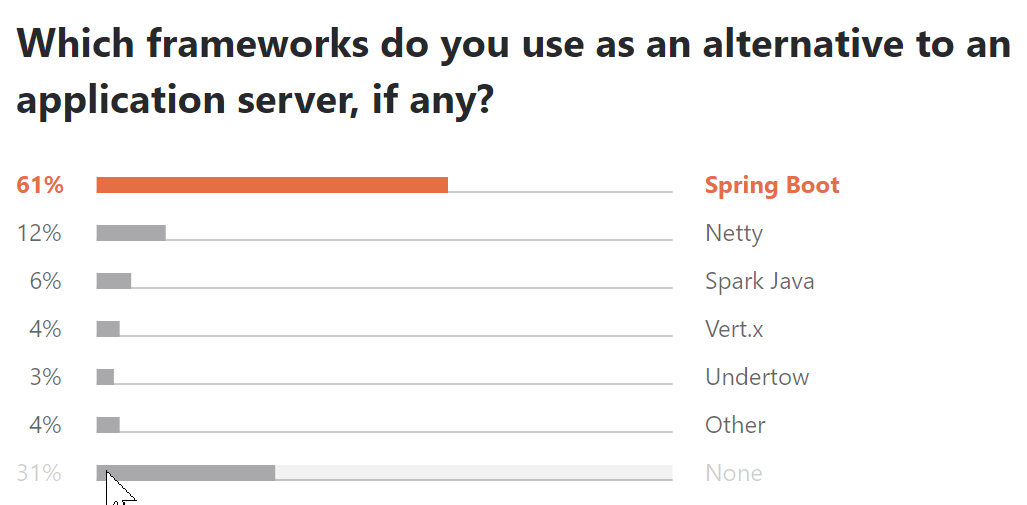
\includegraphics[width=0.75\textwidth]{content/introduction/jb-survey-app-server.png}
    \caption{JetBrains Survey Question About Java Application Server Usage \protect\cite{jetbrains:online}}
    \label{fig:jb-survey-app-server}
\end{figure}

\begin{figure}[H]
    \centering
    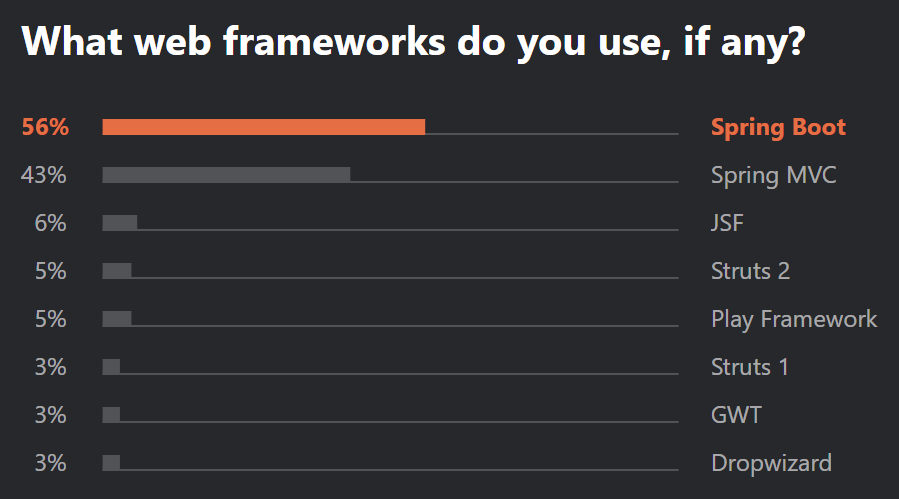
\includegraphics[width=0.75\textwidth]{content/introduction/jb-survey-web-framework.png}
    \caption{JetBrains Survey Question About Java Web Framework Usage \protect\cite{jetbrains:online}}
    \label{fig:jb-survey-web-framework}
\end{figure}

Both questions in the survey were overwhelmingly in favor of Spring Boot so can be easily written with confidence that Spring Boot is a familiar and heavily used Java framework. JetBrains adds that "Spring Boot has become the most popular Java web framework, adding 14\% since last year" \cite{jetbrains:online}.


\section{Architectural Design Approach}

The Spring Boot framework concerns itself with developing web applications quickly and efficiently. Since Spring Boot reuses Spring Framework's codebase for many of its' operations, therefore it is impossible to talk about it without mentioning Spring Framework. The three viewpoints that will be discussed in this document are functional, deployment, and information. The three perspectives cross-cutting these viewpoints are usability, evolution, and development resource.\\

The primary focus for Spring Boot will particularly be the functional viewpoint. Functional viewpoint is important because Spring Boot is an open-source web application framework and relies, in large part, on the contributions from the software community. Spring Boot must maintain a clear description of its functionality and project direction so that contributors can meaningfully contribute. To be able to contribute to Spring Boot, it requires Spring Framework knowledge because much of its inner-workings relies on as a foundation.\\

The deployment viewpoint is important for contributors, maintainers and developers as they need to understand the deployment process for new releases containing features and bug fixes, and eventually where it ends up as an artifact for consumers to source from. It is especially important from the perspective of security since Spring Boot includes many external dependencies that have their own schedule for addressing security vulnerability concerns. Since Spring Boot has an automated build pipeline to release their Spring Boot framework, it brings forth an implicit benefit of speed from development to release. Users are able to get new releases in a timely manner and with these new releases, come new features, enchancements, and fixes.\\

The information viewpoint is important because Spring Boot is primarily about making configuration easier for Spring-based web applications. Knowledge of how Spring Boot enacts auto-configurations requires understanding of how data flows at runtime to create a Spring-based application.


\chapter{Glossary}
{
\obeylines
\setlength\parindent{0pt}

\textbf{GitHub}: Distributed software version control service that offers many features for developer collaboration.\\
\textbf{Repository}: Storage location for software modules.\\
\textbf{Starter Module}: Set of convenient dependencies to include in a Spring Boot web application that follows the naming pattern: \texttt{spring-boot-starter-*} \cite{springbootstarters:online}.\\
\textbf{Module}: Software component which can be used as part of the composition for an application.\\
\textbf{Spring Framework}: Open-source framework that ``Provides a comprehensive programming and configuration model for modern Java-based enterprise applications - on any kind of deployment platform'' \cite{springframework:online}.\\
\textbf{Framework}: Provides capability to create custom application-specific functionality derived from a structured and generic abstraction.\\
\textbf{Servlet Container}: Contained environment on a web server which allows dynamic generation of content on the server-side.\\
\textbf{Servlet}: Java program that runs within a web server that handles requests from web clients over HTTP \cite{servlet:online}.\\
\textbf{BeanFactory}: ''[Inversion of Control] container which instantiates, configures, and manages a number of beans`` \cite{springdefinitions:online}. It is also a subset of the \texttt{ApplicationContext}.\\
\textbf{Bean}: An object instantiated, configured, and managed by the \texttt{BeanFactory}.\\
\textbf{ApplicationContext}: Provides central configuration for a Spring application \cite{springjavadoc:online}.\\
\textbf{Auto-Configuration}: ''Autoconfiguration is a feature that allows library developers to automatically configure beans in the Spring context based on different conditions of the application, such as the presence of certain classes in the classpath, the existence of a bean or the activation of some property`` \cite{springautoconfiguration:online}.\\
\textbf{Classpath}: Parameter in the Java Virtual Machines that identifies class and packages defined by a user \cite{wikiclasspath:online}.\\
\textbf{Soft Link}: References one file to another in a file system, of which when one is changed, the other is as well.\\
\textbf{OpenJDK}: Open-source implementation of Java Standard Edition licensed under GNU General Public License \cite{wikiopenjdk:online}.\\
\textbf{Docker}: Tool that uses the host operating system to package software.\\
\textbf{Artifactory}: Build repository that stores artifacts created from source code.\\
\textbf{Stack Overflow}: Website for professionals in the field of software development to ask and answer questions.\\
\textbf{Lazy Initialization}:  ''When we configure a bean with lazy initialization, the bean will only be created, and its dependencies injected, once they're needed`` \cite{springBootLazyInitialization}.\\
}

\chapter{Stakeholders and Requirements}
\section{Stakeholders}
\subsection*{Acquirers}
Acquirers are decision-makers. Rod Johnson, who started Spring Boot, may be considered its original acquirer. Acquirers are typically concerned with the cost, plan, and return-on-investment; however, since Spring Boot is an open-source framework that is implemented by other projects, the most relevant acquirers, in this case, are the technical directors that approve the implementation of Spring Boot in the project that they oversee.

\subsection*{Assessors}
Assessors are concerned with standards, quality, and compliance with laws and regulations. Maintainers of Spring Boot have implemented automated assessors (Git Hooks and Checkstyles) to ensure that the open-source project maintains a high level of quality. Spring Boot does not, however, have to conform to any legal standards, even if the applications that implement Spring Boot may be regulated.

\subsection*{Communicators}
Communicators are concerned with effectively conveying the purpose and value of a product to its stakeholders. Communicators must have a deep understanding of the system so that they can document it well. Spring Boot documentation is extensive and well maintained by Pivotal, the company that supports the Spring ecosystem, and the project's contributors.

\subsection*{Developers} 
Developers build and deploy software. Spring Boot is a popular open-source project that is maintained by contributors from around the world.

\subsection*{Maintainers}
Maintainers are liable for managing the evolution of the system. Maintainers make sure that the Communicators are up to date on the release documentation. Pivotal developers and Spring Boot contributors are its maintainers.

\subsection*{Production Engineers}
Production engineers are responsible for the management of deployed systems. Because Spring Boot is a framework that is implemented by deployable applications and isn't itself deployed, the project doesn't have production engineers.

\subsection*{Suppliers}
Suppliers provide the third-party software, hardware, and infrastructure required to build, deploy, and maintain a software product. Although Spring Boot is not a deployable application, it does run on the Java Virtual Machine (JVM) and is therefore dependent on the Java Development Kit (JDK). It follows that the Oracle Corporation, which maintains Java, can be considered a supplier to Spring Boot.

\subsection*{Support Staff}
Support Staff are concerned with providing user support. Although Spring Boot is well documented, and there is an extensive community of users that answer questions related to the framework online, the project doesn't have any official Support Staff.

\subsection*{System Administrators}
System Administrators are in charge of monitoring and management of the system once it has been deployed to production. Although Spring Boot applications need System Administrators, the Spring Boot project does not.

\subsection*{Testers}
Testers are responsible for testing the system to verify the correctness of the product and its specifications. Spring Boot contributors are responsible for testing their code. Spring Boot does not seem to have a dedicated group of testers.

\subsection*{Users}
Users are in charge of defining the functional requirements of a system. Spring Boot users are Java developers that build web services.
\section{Overview of Requirements}
\subsection{Functional Requirements}

\begin{table}[H]
    \begin{tabular}{l p{13cm}}
    F-01 & The Spring Boot module shall be able to independently embed servlet containers.\\\\
    F-02 & The Spring Boot module shall be able to retrieve application metrics over the network.\\\\
    F-03 & The Spring Boot module shall be able to perform auto-configuration through scanning libraries in the classpath.\\\\
    F-04 & The Spring Boot module shall give priority to declared properties for configuration above all auto-configuration.\\\\
    F-05 & The Spring Boot module shall use Logback as the default logging framework when a logging framework dependency is not defined in the classpath.\\\\
    F-06 & The Spring Boot module shall be able support external dependency management tools to build artifacts.\\\\
    F-07 & The Spring Boot framework shall contain starter modules with pre-configured dependencies.\\\\
    F-08 & The Spring Boot module shall be able to auto-restart when any file on the classpath are changed and spring-boot-devtools is present in the classpath.\\\\
    F-09 & The Spring Boot module shall integrate with multiple caching mechanisms.\\\\
    F-10 & The Spring Boot website shall be able to auto-generate dependencies for external dependency management tools with user-specified properties.
    \end{tabular}
\end{table}
\subsection{Non-functional Requirements}

\begin{table}[H]
    \begin{tabular}{l p{13cm}}
    NF-01 & The software shall integrate with multiple caching mechanisms.\\\\
    NF-02 & The software shall allow for the autonomous scaling of servers to any environment without interruption to service.\\\\
    NF-03 & The software shall have a written set of guidelines for project contribution.\\\\
    NF-04 & The software shall allow for asynchronous processes.\\\\
    NF-05 & The software shall support integration with external infrastructure technologies.\\\\
    NF-06 & The software shall log all issues in the default configuration library.\\\\
    NF-07 & The software shall be extensible.\\\\
    NF-08 & The software shall integrate with external authentication technologies.\\\\
    NF-09 & The software documentation shall list available internal libraries with each new release.\\\\
    NF-10 & The software documentation shall contain descriptions of new features with each new release.\\\\
    NF-11 & The software documentation shall be up-to-date with each new release.\\\\
    NF-12 & The software shall not constrain users to any coding style.                                        
    \end{tabular}
    \end{table}
\section{System Scenarios}
\subsection{Functional Scenarios}

\subsection*{Spring Boot Application Context Creation}

\textbf{Overview:} How Spring Boot creates the application context.\\

\textbf{System state:} No web application type specified and application is using the \texttt{spring-boot-starter-web} module \\

\textbf{System environment:} Local machine is running as normally and integrated development environment is fully functional. \\

\textbf{External stimulus:} The \texttt{SpringApplication.run()} method is invoked. \\

\textbf{Required system response:} The Spring Boot application by default -- if the web application type \texttt{SERVLET} or \texttt{REACTIVE} are not specified as a context -- will create a new \texttt{ApplicationContext} instance off of the\\ \texttt{org.springframework.web.context.support.AnnotationConfigApplicationContext}\\ class and return it. The allows the user to be given an \texttt{ApplicationContext} without having to manually define a configuration.

\subsection*{Dependency Auto-configuration}

\textbf{Overview:} How Spring Boot deciphers what to auto-configure based on dependencies in the classpath.\\

\textbf{System state:} All desired dependencies from the starter modules are declared appropriately in the chosen dependency management tool. The \texttt{Main} application class has been annotated with \texttt{@SpringBootApplication}. \\

\textbf{System environment:} Local machine is running as normally and integrated development environment is fully functional. \\

\textbf{External stimulus:} The \texttt{SpringApplication.run()} method is invoked. \\

\textbf{Required system response:} The Spring Boot application will iterate over the collection of \texttt{spring.factories} auto-configuration classes, in which it will scan dependencies declared in the classpath to find all matches. Once the dependencies have been discovered for matches, they will be auto-configured accordingly.

\subsection*{Spring Boot Conditional Annotation}

\textbf{Overview:} How Spring Boot allows custom conditionals to apply configurations.\\

\textbf{System state:} The \texttt{Main} application class has been annotated with \texttt{@SpringBootApplication}. A custom configuration class has been created and annotated with the \texttt{@Configuration} from \texttt{org.springframework.context.annotation} and \texttt{@ConditionalOnClass} from \texttt{org.springframework.boot.autoconfigure.condition} containing a specified classname as an argument. \\

\textit{Note: There are other available conditional annotation classes}\\

\textbf{System environment:} Local machine is running as normally and integrated development environment is fully functional. \\

\textbf{External stimulus:} The \texttt{SpringApplication.run()} method is invoked. \\

\textbf{Required system response:} The Spring Boot application will use the spring framework to scan custom configuration classes and then check whether the \texttt{@ConditionalOnClass} is met. This is done by calling the \texttt{OnClassCondition} class, which in itself uses the \texttt{getMatchOutcome} function that resolves to returning a \texttt{ConditonOutcome} object containing a boolean and message. If the condition is met, then the logic within the custom configuration class will be used.

\subsection*{Custom Failure Analyzer}

\textbf{Overview:} How Spring Boot allows implementation of custom failure analyzers on failed application start-up.\\

\textbf{System state:} The \texttt{Main} application class has been annotated with \texttt{@SpringBootApplication}. A custom implementation of the \texttt{FailureAnalyzer} interface has been created and the \texttt{analyze()} method has been overridden. The Spring Boot application is unable to start. \\

\textbf{System environment:} Local machine is running as normally and integrated development environment is fully functional. \\

\textbf{External stimulus:} The \texttt{SpringApplication.run()} method is invoked. \\

\textbf{Required system response:} The Spring Boot application on start-up failure will run the \texttt{analyze()} method which will be called automatically by Spring Boot. The method will return new \texttt{FailureAnalysis} objects that requires arguments of \texttt{custom failure message}, and \texttt{Throwable} based on the custom \texttt{FailureAnalyzer} implementation. Those objects are surfaced to the console to display to the user as an explanation as to why the start-up of the application failed.

\subsection*{Conditional Evaluation Reporting at Runtime}

\textbf{Overview:} How Spring Boot creates a \texttt{conditional evaluation report} when application fails at the start-up due to a conditional non-match of a declared bean.\\

\textbf{System state:} The \texttt{Main} application class has been annotated with \texttt{@SpringBootApplication}. The Spring Boot application is not able to start up. There is a custom bean declared with \texttt{@ConditionalOnProperty} and there is no property that exists to match the condition. The log level is set to DEBUG. \\

\textbf{System environment:} Local machine is running as normally and integrated development environment is fully functional. \\

\textbf{External stimulus:} The \texttt{SpringApplication.run()} method is invoked. \\

\textbf{Required system response:} The Spring Boot application uses the \texttt{ConditionEvaluationReportLoggingListener} class under the package\\ \texttt{org.springframework.boot.autoconfigure.logging}, which contains a method called \texttt{onApplicationEvent} that eventually calls a method called \texttt{logAutoConfigurationReport}. This method will resolve to evaluating whether or not the log level is set to DEBUG and if it is, then there will be an output displayed in the console based on the \texttt{ConditionEvaluationReportMessage} class' resolution. 

\subsection{Quality Scenarios}

\subsection*{Performance}

\textbf{Overview:} Check the Spring Boot application start-up time responsiveness.\\

\textbf{System and environment state:} The Spring Boot application has all dependencies defined as well as one HTTP endpoint. The application is able to start up with no errors.\\

\textbf{External stimulus:} Developer runs the Spring Boot application.\\

\textbf{System response:} Spring Boot's latest release uses global lazy initialization to reduce the time to start-up an application by creating bean objects only when it is needed.\\

\textbf{Response measure:} In 95\% of Spring Boot application start-up will start up in less than one second. In 99.9\% of application start-up, it will start up within one second.


\subsection*{Usability}

\textbf{Overview:} Spring Boot takes an opinionated stance of auto-configuring all dependency details by default. \\

\textbf{System and environment state:} The Spring Boot application has all starter dependencies defined in the dependency management tool. The application is able to start up with no errors. \\

\textbf{External stimulus:} Developer runs the Spring Boot application. \\

\textbf{System response:} Spring Boot will use auto-configuration classes to configure dependencies from the classpath. \\

\textbf{Response measure:} In 95\% of all instances, Spring Boot requires less effort than a Spring MVC application.


\subsection*{Security}

\textbf{Overview:} Check how the Spring Boot application handles invalid user credentials.\\

\textbf{System and environment state:} The \texttt{spring-boot-starter-security} has been defined as a dependency, and Spring's content negotiation strategy is implementing HTTP Basic authentication \cite{springBootSecurity}. The system is using the default \texttt{SecurityAutoConfiguration} class. The system is operating under its definition of normal load, has deployed without error, and is communicating over a good internet connection.\\

\textbf{External stimulus:} A user sends a \texttt{GET} request with an invalid username and password in its header.\\

\textbf{System response:} The system returns a \texttt{401 Unauthorized} response to the \texttt{GET} request.\\

\textbf{Response measure:} Invalid credentials always trigger a \texttt{401 Unauthorized} response.


\subsection*{Supportability}

\textbf{Overview:} How Spring Boot help identify issues in start-up of consuming project. \\

\textbf{System and environment state:} The integrated development environment is fully functional and the Spring Boot application is not able to start-up because it could not satisfy the condition to instantiate a bean that is being used in application. \\

\textbf{External stimulus:} Developer runs the Spring Boot application. \\

\textbf{System response:} Spring Boot uses default logging of logback for the errors that might come during the start-up. In this case, the Spring Boot will find the error and report back to the consuming project. \\

\textbf{Response measure:} In 95\% of Spring Boot application start-up will report the error in less than one second. In 99.9\% of application start-up, it will report within one second.

\subsection*{Reusability}

\textbf{Overview:} Developer adds new component to Spring Boot project that did not exist before by leveraging existing components. \\

\textbf{System and environment state:} Spring Boot project is downloaded and loaded in the integrated development environment. The integrated development environment is working with no errors. \\

\textbf{External stimulus:} Developer adds support for new component to enable lazy initialization globally by providing new annotation/interface. \\

\textbf{System response:} Spring Boot will be able to provide support for global lazy initialization exposed through annotation reusing existing components. \\

\textbf{Response measure:} In 95\% of all instances, Spring Boot requires less effort to write the new component by leveraging the existing component as Spring Boot follows the principal of separation of concern wisely.

\chapter{Architectural Forces}
\section{Goals}

Spring Boot has the following goals:

\begin{itemize}
\item Usability -- Sprint Boot framework is developed with the intention of assisting developers auto-configure dependencies and quickly build out a web application. The framework helps developers to avoid spending time learning and understanding how to configure dependencies as compared to Spring Framework. The Spring Framework essentially forces a user to configure dependencies themselves by mechanism of specific annotation declarations with written java code, or XML configurations.
\item Efficiency -- Developers spending less time on basic configurations and writing redundant code ultimately results in increased productivity, and gives the ability to get a business product to production faster.
\item Development Resource -- The Spring Boot framework underneath the good uses the Spring Framework as its' foundation but it also brings along unique qualities and characteristics. Since the Spring ecosystem is so large and complex, this requires meticulous dedication to learn it in-and-out to contribute in a way that allows it to be maintainable, scalable, and meaningful to its' community.
\end{itemize}

\section{Constraints}

Spring Boot has the following constraints:

\begin{itemize}
\item Spring Boot is written in Java and uses the \texttt{Spring Java Format} which enforces Spring-specific code formatting conventions for contributors \cite{springBootContribution}.
\item Spring Boot requires embedded servlet containers such as Tomcat, Jetty, and Undertow to support the deployment of applications.
\item Spring Boot takes an opinionated view of utilizing Spring Framework to its advantage and therefore its evolution is directly tied to it.
\item Sprint Boot makes dependency management of third party libraries easier by integrating common libraries into its' module as transitive dependencies. Some of these common transitive dependencies include logging frameworks like SLF4J and Log4J, serializer and deserializer such as GSON and Jackson, and databases such as MongoDB and PostgreSQL.
\end{itemize}

\section{Architectural Principles}

\noindent\makebox[\linewidth]{\rule{\textwidth}{3pt}}\ \\

\textbf{Principle}: The Spring Boot framework when used within a consuming project must greatly minimize the effort of writing configurations for developing a Spring-based web application.\\

\textbf{Rationale}: If Spring Boot does not reduce the effort for Java developers to write boilerplate configuration code, it will not have a convincing reason to be adopted over Spring Framework or other web application frameworks.\\

\textbf{Implications}: 
\begin{itemize}
\item Spring Boot must use Spring Framework as its' foundation.
\item Spring Boot must be written in Java or other JVM-based programming languages.
\item Spring Boot must abstract away all configuration code into a simple interface from the perspective of a Java developer.
\item A consuming project must be able to use short, expressive, and single-lined annotation abstractions to auto-configure all class path dependencies.
\item A consuming project must have a way to pre-define objects to be configured by code that is understood by Spring Boot.
\item Spring Boot features and documentation must be up to date with software technology trends to stay relevant to Java developers.
\end{itemize}

\noindent\makebox[\linewidth]{\rule{\textwidth}{3pt}}\ \\

\textbf{Principle}: The Spring Boot framework when used within a consuming project must be able to delivery value to the wide-ranged use cases of Java developers within the context of web application development.\\

\textbf{Rationale}: Java Developers all have unique situations, circumstances, and environments of which they work in. There is no one-size-fits-all type of framework so Spring Boot has to justify their flexibility and adaptability to tend to the needs of Java developers.\\

\textbf{Implications}: 
\begin{itemize}
\item Spring Boot must be able to integrate with a wide range of external libraries concerning web application development.
\item Spring Boot must be able to acknowledge and address the concerns of integration with other libraries.
\item Spring Boot must package commonly used and cohesive libraries together to address a particular need.
\item Spring Boot must be easily accessible to Java developers through a repository.
\end{itemize}

\noindent\makebox[\linewidth]{\rule{\textwidth}{3pt}}\ \\

\textbf{Principle}: The Spring Boot framework must be developed by reusing many functionalities of the Spring Framework.\\

\textbf{Rationale}: Code reuse is a large part of developing software to reduce redundancy and shorten development time.\\

\textbf{Implications}: 
\begin{itemize}
\item Spring Boot must adhere to some the design constraints of Spring Framework.
\item Spring Boot must work in harmony with Spring Framework and not against it.
\item Spring Boot must be able to market itself apart from Spring Framework.
\item Spring Boot must offer something to Java developers that Spring Framework already does not.
\end{itemize}

\noindent\makebox[\linewidth]{\rule{\textwidth}{3pt}}


\chapter{Architectural Views Top Level}
\section{Perspectives}

\subsection{Usability}
The usability of Spring Boot is promoted by abstracting complex functions into annotations that are available to use by Java developer. Developers are champions in advocating for simple and reusable code, and this is where Spring Boot shines. From their perspective, it does not matter how Spring Boot internally works, but what it offers them to make their web application development efforts easier. Although this may sound great -- as with any new framework -- there is a learning curve to understand how to properly use and integrate it with an application. Spring in general however, is a extremely familiar software ecosystem to the Java development community. There is an abundant amount of Spring Boot resources such as videos, articles, blogs, forums, and other media platforms to learn from. This is in addition to the availability of Spring Boot maintainers that can answer questions and address concerns through GitHub and Stack Overflow. This is undoubtedly one of the reasons why Spring Boot is popular amongst Java developers and why they may choose to use it over other similar frameworks.\\

Java developers should be able to easily use Spring Boot framework once they understand the high level idea of how it works. That is to say, to understand on the high level what the annotations do and how they relate to one another when applying them to code.

\subsection{Evolution}
The evolution perspective has little to no impact on the deployment viewpoint, but has large implications on Spring Boot from a functional viewpoint. The direction from which the framework has to be adjusted is heavily in the hands of its' community of users, as the framework itself is open-source project. The features that are developed, enhancements that are made to give a better development experience, and fixes that patch bugs and vulnerabilities are all community-driven but ultimately addressed by the Spring Boot team. The Spring Boot team are the assessors of the trade-offs of every change requested from the community; they have to carefully consider every potential consequence of changes, the benefits, and the opportunities it opens up for the future.\\

For example, the decision to create the Spring Boot project was out of the common frustration to write boilerplate configuration as code, when it could just have been automated to avoid the frustration altogether. The implication of this however is that users are unaware of the Spring Boot magic behind why their web applications just works, so there is ignorance on behalf of the user. This ignorance can manifest itself in many ways, one of which the user does not understand why most dependencies are auto-configured and some are not. As users of Spring Boot, they would have to dig into the code and be hassled with the immense complexity to figure out why certain dependencies were not auto-configured or ask the larger Spring Boot community. The huge upside simply, is that it just works for most situations regardless of whether the user has thorough understanding of the internal workings of Spring Boot or not. The bigger idea here, is that when the issues arise with using the Spring Boot framework, the user typically will be lost and look to the community at large. That is the trade-off with abstraction.\\

The Spring Boot architecture is reliant on external dependencies. It therefore is nothing without the existence of those external dependencies because it's primary job is to auto-configure them. To put it another way, the architectural evolution of Spring Boot is directly tied to libraries outside of its' control. The way the code is written to auto-configure those libraries is up to the way they were developed.

\subsection{Development Resource}
Development resource is extremely important to the functional viewpoint because of the complexity of abstraction of Spring Boot's code. For a person to be able to meaningfully contribute to the core of the codebase, a developer in the Spring Boot team has to understand how Spring Boot internally works. It requires that the person understands how to utilize design patterns in specific situations to implement new code, let alone how to read code to understand the design patterns going on in the codebase. This also touches on the understanding of the information viewpoint because of the runtime data flow within the Spring Boot framework to auto-configure dependencies. Both of these viewpoints affects how a developer would refactor, extend, and design the codebase for sustainability and maintainability. For the deployment viewpoint, a developer must have special knowledge on system engineering, creating automated pipelines to achieve the goal of deploying the Spring Boot framework confidently, effectively, and efficiently. This is all the more important since it is a framework used by so many developers around the world, so there is quite an impact when done incorrectly. All of this requires a developer have quite expansive knowledge no matter where they may specialize within the Spring Boot team. To bring a new developer up to speed may require a lot of time, let alone the rigorous coding standards that the team imposes on the development of the framework.

\section{Context View}

\begin{figure}[ht]
    \centering
    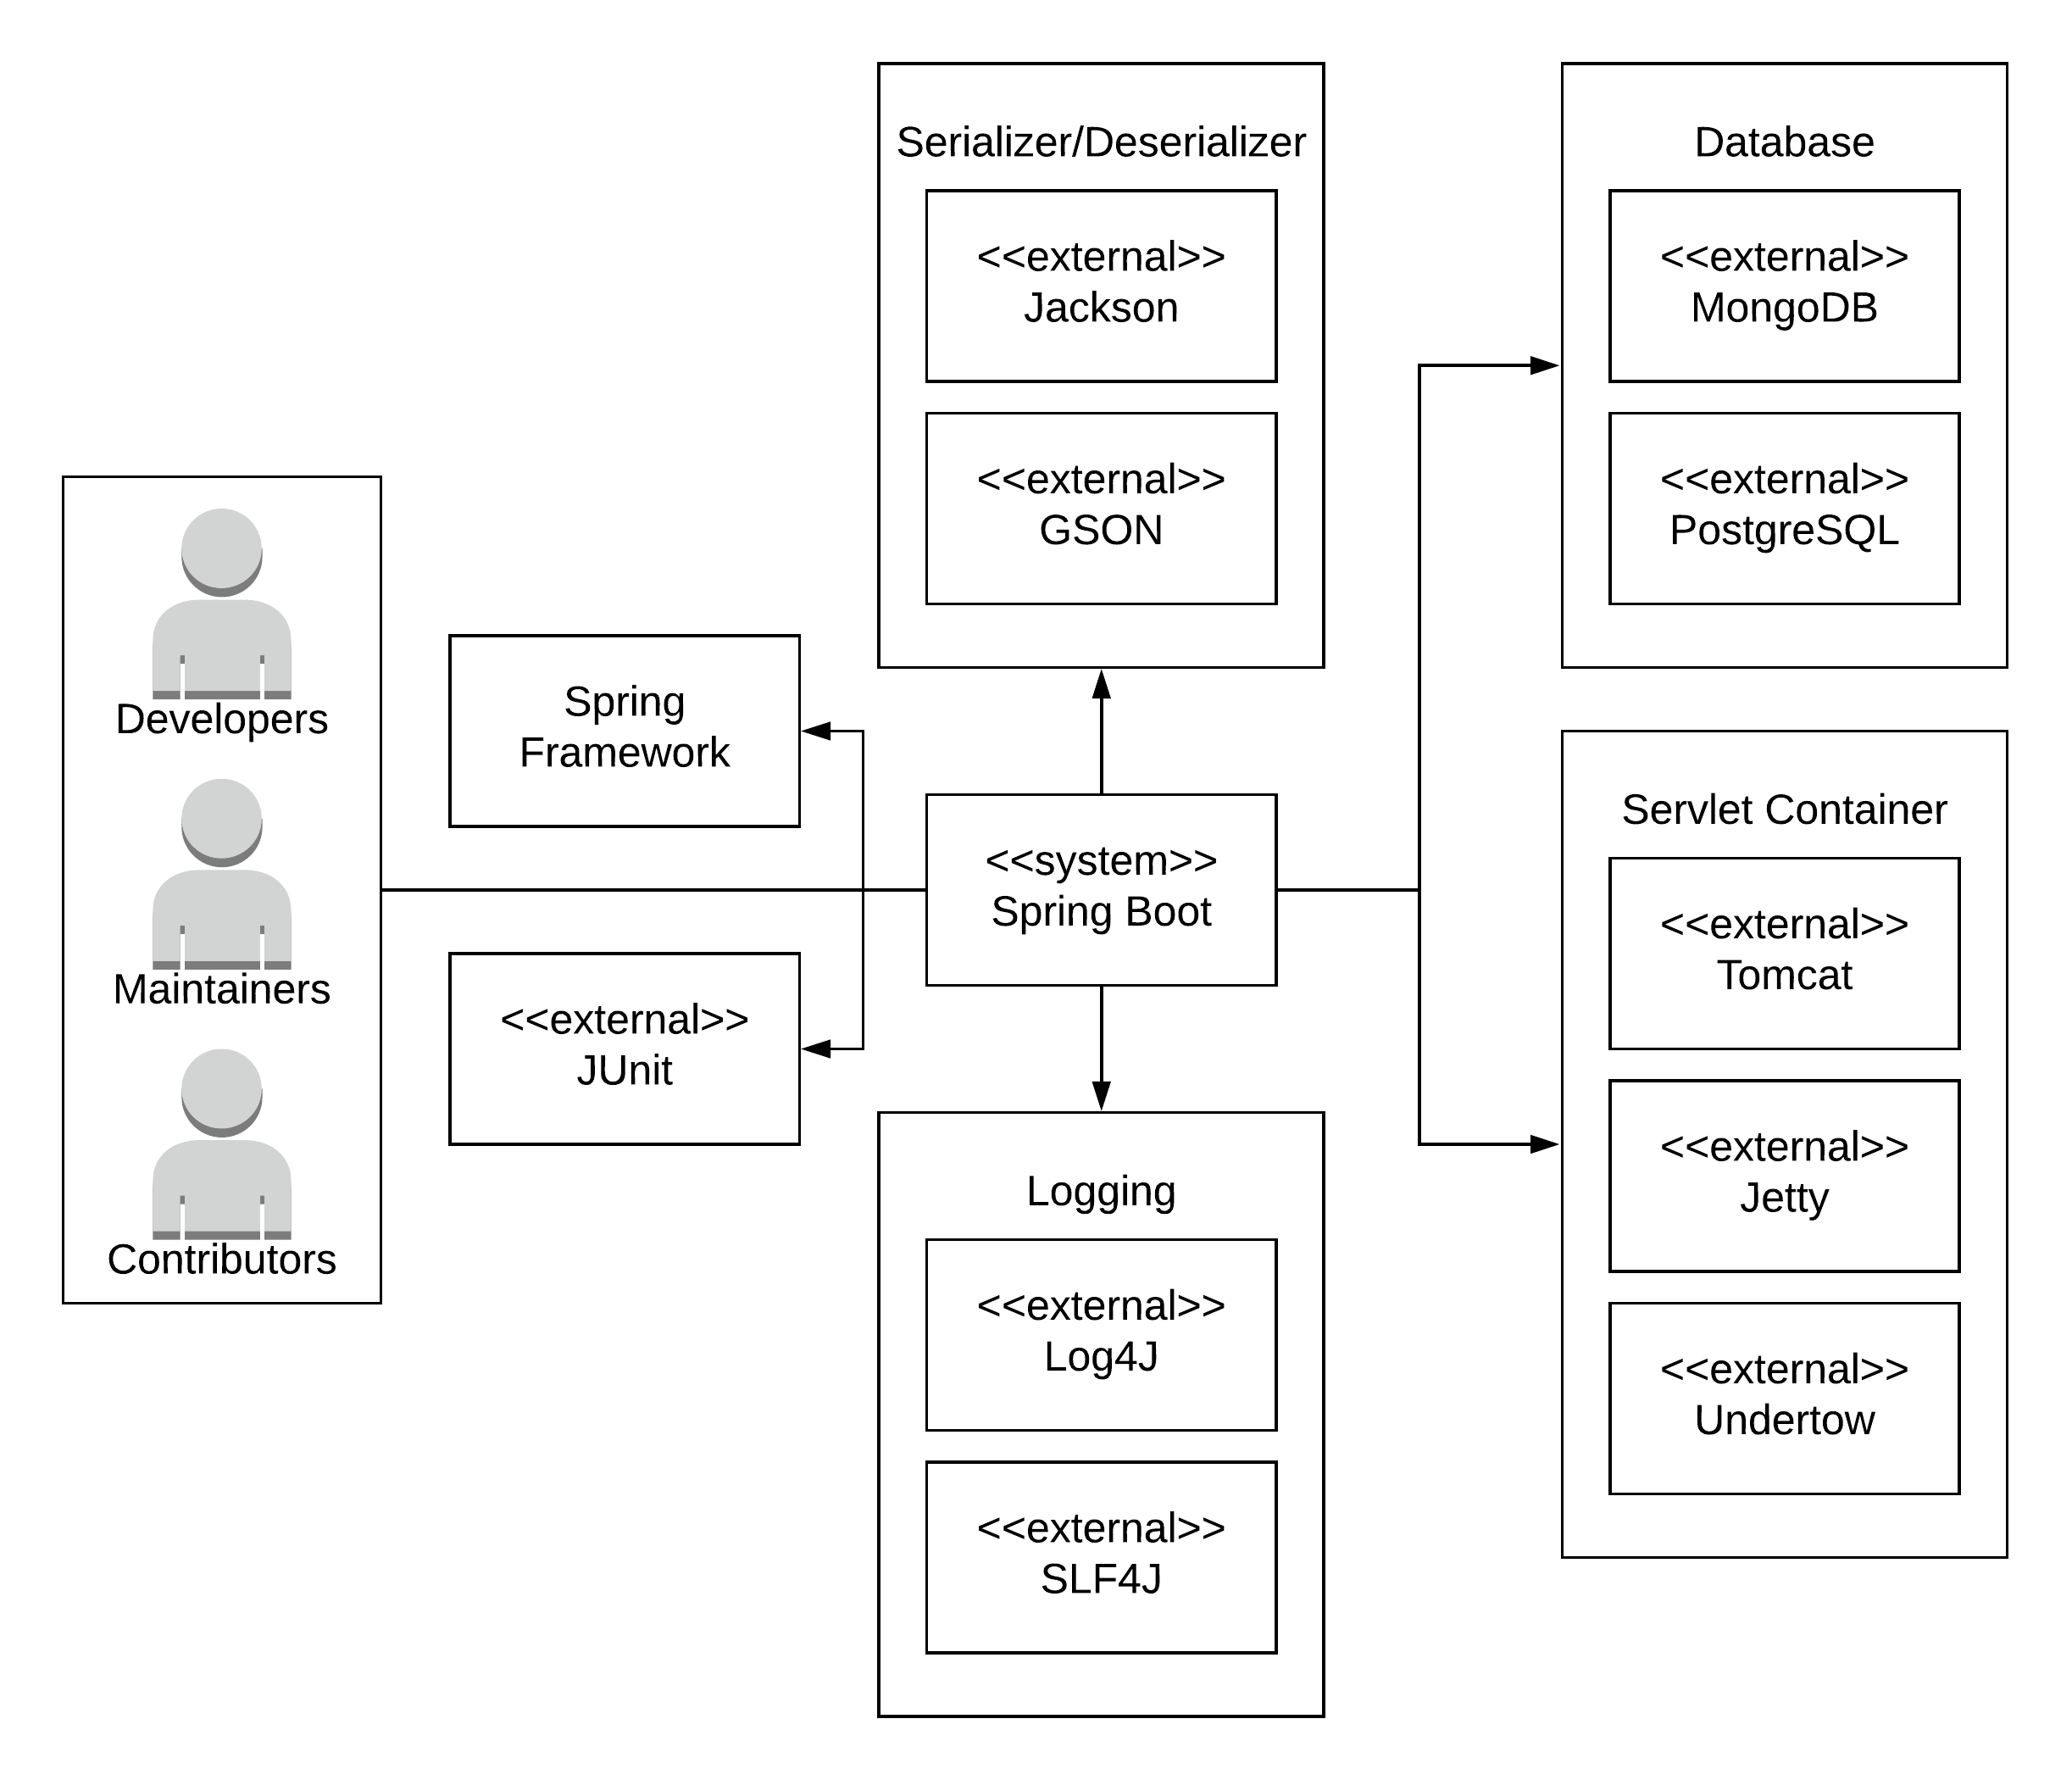
\includegraphics[width=0.75\textwidth]{content/architectural-views-top-level/context-diagram-spring-boot.png}
    \caption{Spring Boot Context Diagram}
    \label{3-context-diagram}
\end{figure}

Spring Boot has the following actors, which are listed below:

\begin{enumerate}
  \item \textbf{Developers}: Users who develop web service applications using Spring Boot.
  \item \textbf{Maintainers}: The team that overlooks the open-source Spring Boot project and develops features as well as addressing bugs and vulnerabilities.
  \item \textbf{Contributors}: The Spring community at wide that participates in improving, developing, and reporting bugs and vulnerabilities.
\end{enumerate}

Spring Boot has the following dependencies, which are listed below:

\begin{enumerate}
  \item \textbf{Spring Framework}: A Java-specific platform for developing a wide-range of applications.
  \item \textbf{JUnit}: A Java-specific testing framework for unit and integration testing
  \item \textbf{Logging}: Spring Boot has logging integration for libraries such as Log4J and SLF4J, which can provide various logging levels dependent on user informational needs (i.e. \texttt{OFF, FATAL, ERROR, WARN, INFO, DEBUG, TRACE}).
  \item \textbf{Servlet Containers}: Spring Boot by default supports three embedded servlet containers such as Tomcat, Jetty, Undertow. These containers have the ability to communicate via HTTP protocols from client to servlet.
  \item \textbf{Database}: Spring Boot has support for a variety of database systems such as MongoDB and PostgreSQL.
  \item \textbf{Serializer/Deserializer}: Spring Boot by default uses Jackson to serialize and deserialize but can use other libraries such as GSON and custom implementations

  \textit{Note: The list is not exclusive to the above list and more dependencies can be found in the official Maven repository}
\end{enumerate}

Spring Boot has six internal key components, which are listed below:

\begin{enumerate}
  \item \textbf{Actuator}: additional features to monitor and manage a Spring application in production.
  \item \textbf{Autoconfigure}: automatically configures the Spring application based on the jar dependencies.
  \item \textbf{CLI}: command-line interface for developing Spring applications.
  \item \textbf{Starters}: dependency descriptors required to enable additional Spring functionality.
  \item \textbf{Test}: annotations and utilities for testing.
  \item \textbf{Tools}: additional development support features like LiveReload.
\end{enumerate}
\section{Functional View}

\begin{figure}[H]
    \centering
    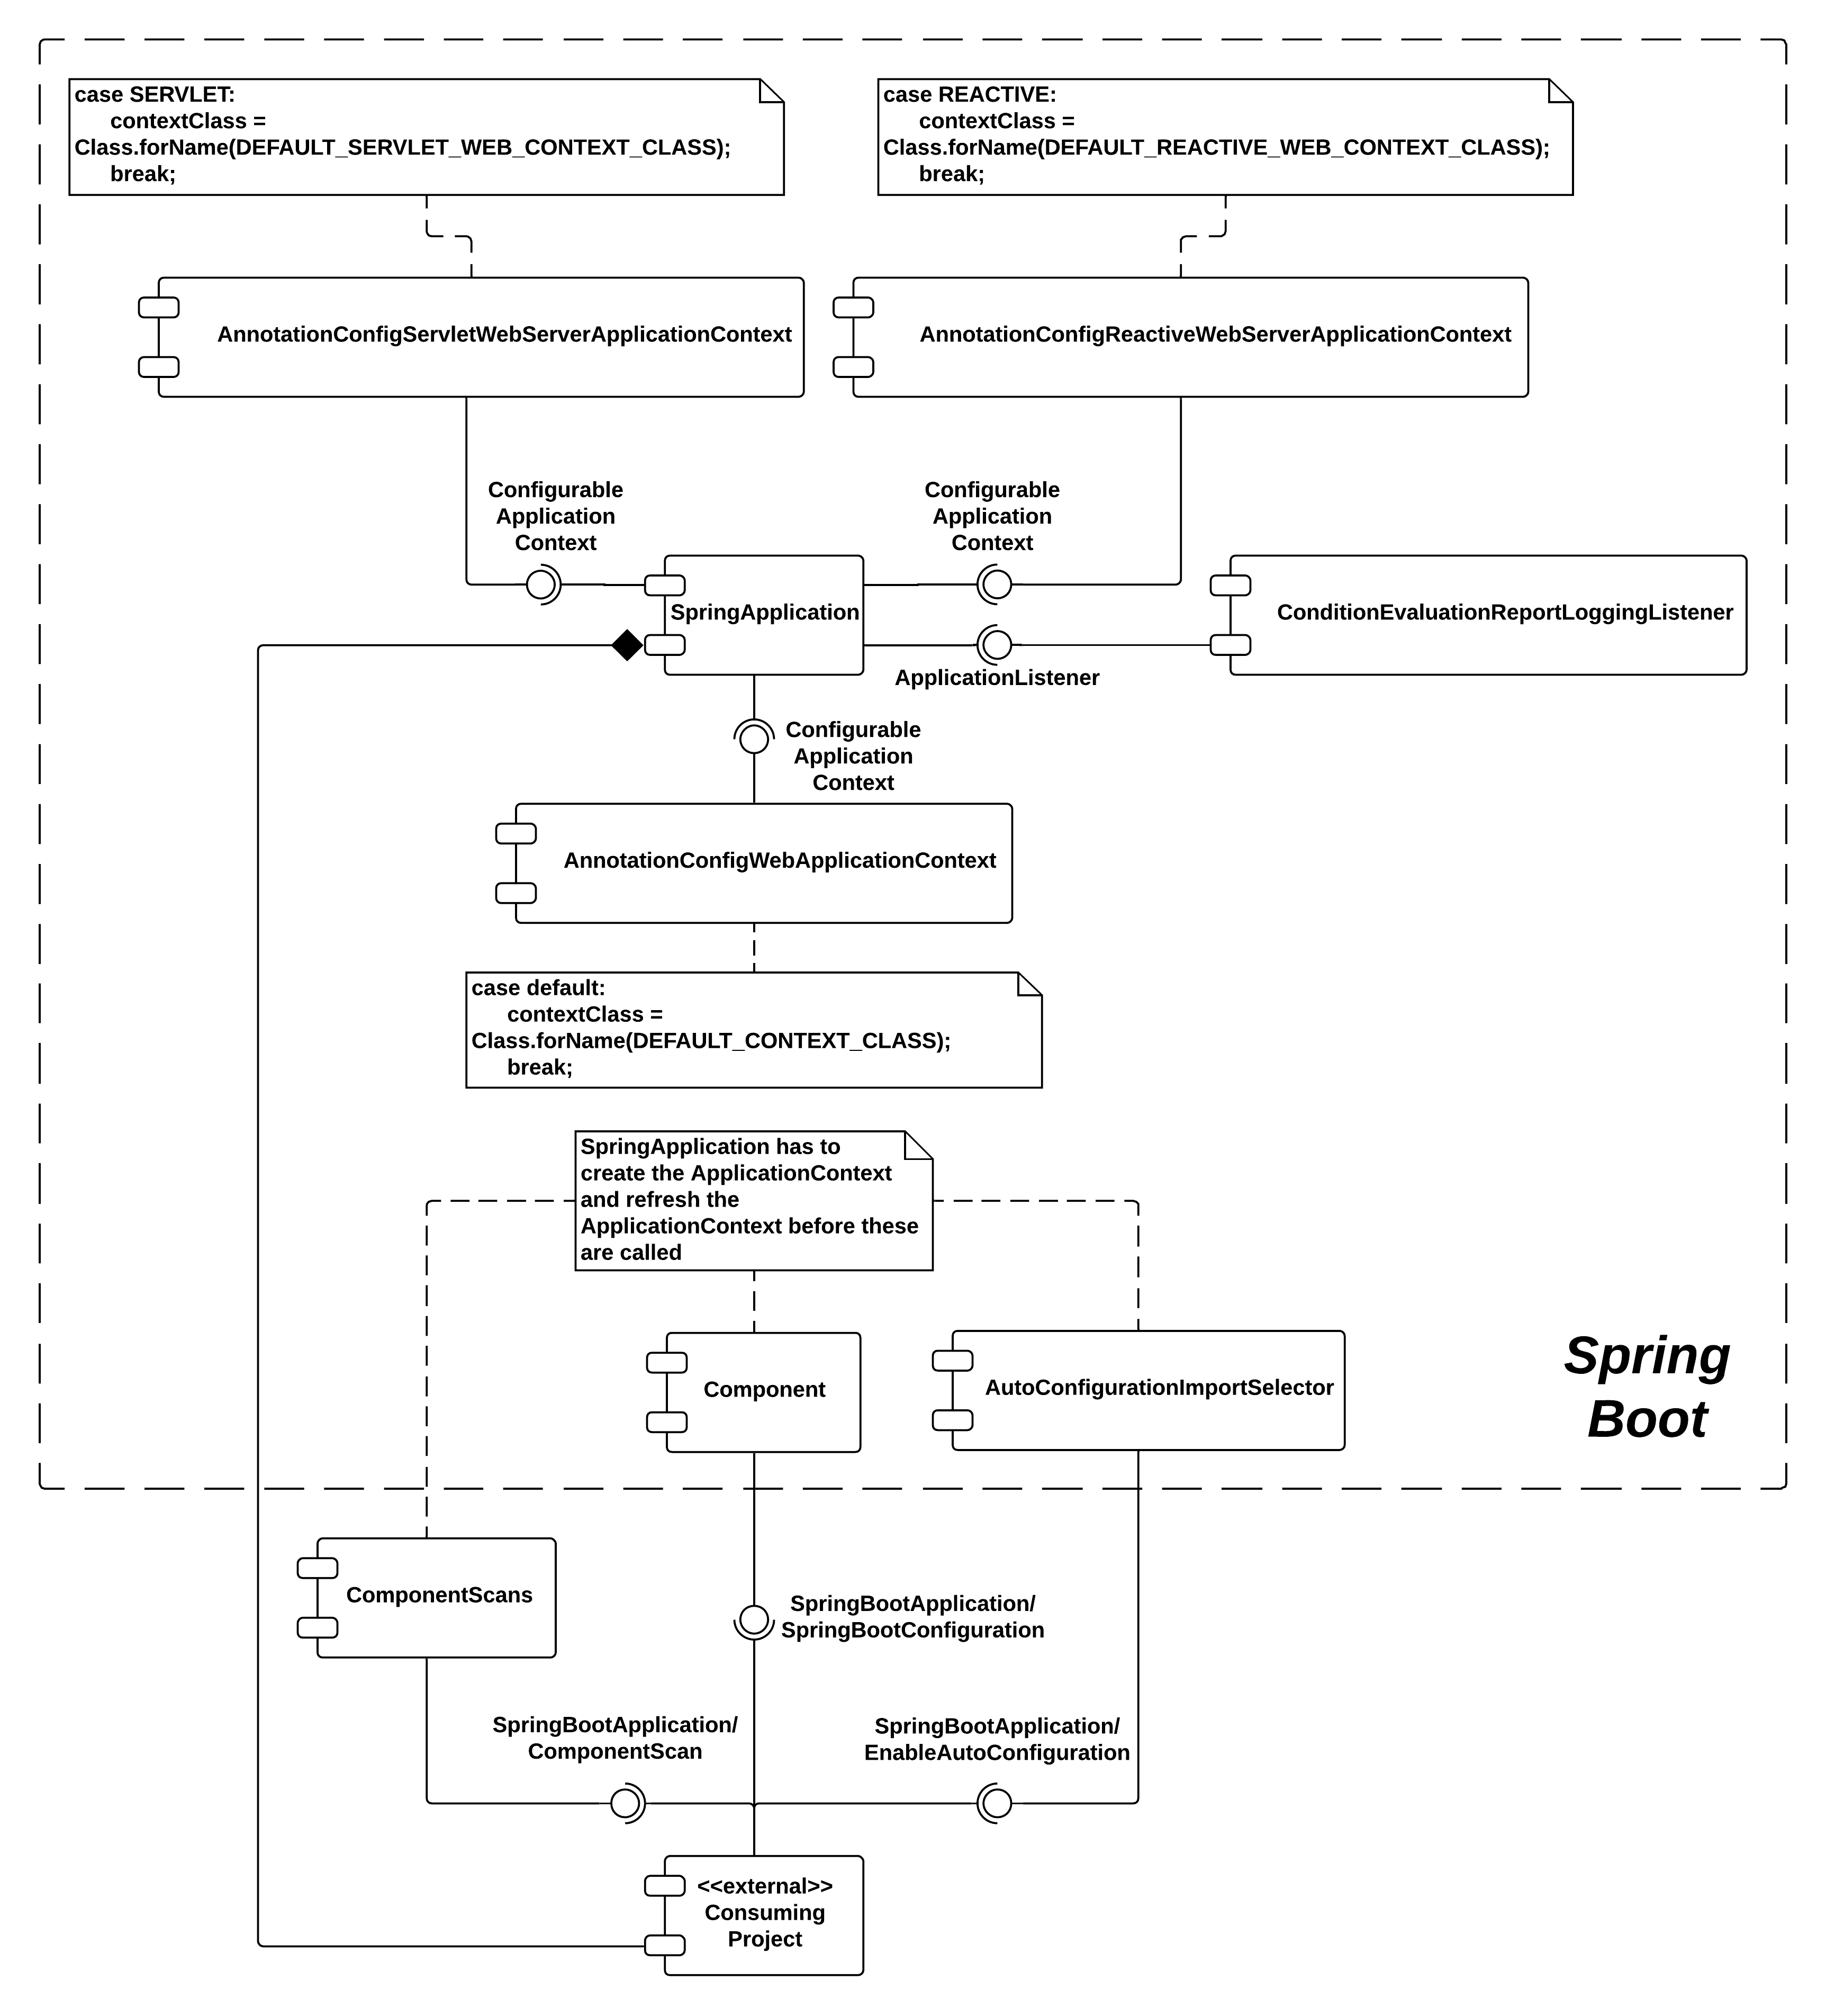
\includegraphics[width=.9\textwidth]{content/architectural-views-top-level/spring-boot-component-diagram.png}
    \caption{Spring Boot Component Diagram}
    \label{component-diagram}
\end{figure}

Spring Boot leverages some functionalities of Spring Framework and takes an opinionated stance of building Spring web applications. It is important to point out the opinion of Spring Boot, because this is the primary reason that it removes the burden of developing boilerplate configurations.  It does so with the \texttt{@SpringBootApplication} annotation that extends the interfaces -- EnableAutoConfiguration, SpringBootConfiguration and ComponentScan -- to give the user an easier experience for setting up a web application. They do not have to completely understand the magic that happens behind the scene but reap the benefit of the abstraction.

Spring Boot enacts the following tasks in sequence when a consuming project initiates a start-up using \texttt{SpringApplication.run()}:

\begin{enumerate}
\item The application context starts.
\item A component scan occurs with the \texttt{@ComponentScan} annotation -- which is a functionality of Spring Framework -- and discovers all subpackages relative to the consuming project's application class.
\item The \texttt{@SpringBootConfiguration} annotation will use the discovered subpackages as its' scope for instantiating and configuring pre-defined beans within it.
\item The \texttt{@EnableAutoConfiguration} annotation instantiate beans based on the dependencies in the classpath. It will also match the dependencies in the classpath and compare it to the \texttt{spring.factories} properties, which then evaluates conditionals based on a match to check whether auto-configuration is necessary.
\end{enumerate}

\subsection{Functional Elements}

As a reference point for Listings~\ref{AnnotationConfigServletWebServerApplicationContext},~\ref{AnnotationConfigReactiveWebServerApplicationContext}, and~\ref{AnnotationConfigApplicationContext}, Listing~\ref{ApplicationContext} shows Spring Boot's code that contains a Java switch case statement which determines the application context based on the web application type of the consuming project. To give a little more context, the web application type is deduced from the classpath dependencies. On a high level, each of the application context are resolved to with the following in their classpath:

\begin{itemize}
\item \texttt{javax.servlet.Servlet} or\\\texttt{org.springframework.web.context.ConfigurableWebApplicationContext} resolves to a \texttt{SERVLET} application context.
\item \texttt{org.springframework.web.servlet.DispatcherServlet} resolves to a \texttt{REACTIVE} application context.
\item If none of the above are present in the classpath, Spring Boot will resolve to a default application context.
\end{itemize}

\clearpage

\begin{lstlisting}[language=Java, caption={Determination of Application Context \cite{createapplicationcontext:online}}, label=ApplicationContext]

protected ConfigurableApplicationContext createApplicationContext() {
	Class<?> contextClass = this.applicationContextClass;
	if (contextClass == null) {
		try {
			switch (this.webApplicationType) {
			case SERVLET:
				contextClass = Class.forName(DEFAULT_SERVLET_WEB_CONTEXT_CLASS);
				break;
			case REACTIVE:
				contextClass = Class.forName(DEFAULT_REACTIVE_WEB_CONTEXT_CLASS);
				break;
			default:
				contextClass = Class.forName(DEFAULT_CONTEXT_CLASS);
			}
		}
		catch (ClassNotFoundException ex) {
			throw new IllegalStateException(
					"Unable create a default ApplicationContext, please specify an ApplicationContextClass", ex);
		}
	}
	return (ConfigurableApplicationContext) BeanUtils.instantiateClass(contextClass);
}
	
\end{lstlisting}\ \\

The following are the list of most common functional elements of Spring Boot:
{
\obeylines
\setlength\parindent{0pt}

\noindent\makebox[\linewidth]{\rule{\textwidth}{3pt}}\ \\

\textbf{Element Name}: AutoConfigurationImportSelector\\
\textbf{Description}: AutoConfigurationImportSelector uses an interface called EnableAutoConfiguration. The EnableAutoConfiguration interface is extended by the SpringBootApplication interface, which uses the auto-configuration classes inside of the \texttt{spring.factories} properties and are applied based on dependencies in the classpath. This mechanism for applying the auto-coonfigurations is done through the \texttt{SpringFactoriesLoader} class under the \texttt{org.springframework.core.io.support} package which iterates over \texttt{spring.factories} file properties living inside of the \texttt{org.springframework.boot.autoconfigure} package. The iteration process is looking for matches to the Auto-configuration classes, then evaluates the conditionals in each of those matching classes such as \texttt{@ConditionalOnClass}. EnableAutoConfiguration also has ways in which users can exclude any configuration that do not need to be applied. There are two ways to exclude auto-configuration of specific dependencies by using the \texttt{exclude()} and \texttt{excludeName()} methods within EnableAutoConfiguration.\\
\textbf{Interface}: The consumer project's application class with the \texttt{main} method that invokes \texttt{SpringApplication.run()}:\\

\begin{lstlisting}[language=Java, caption=Consumer Project Auto-Configuring Dependencies using SpringBootApplication]

import org.springframework.boot.autoconfigure.mongo.MongoAutoConfiguration;
import org.springframework.boot.autoconfigure.data.mongo.MongoDataAutoConfiguration;
import org.springframework.boot.SpringApplication;
import org.springframework.boot.autoconfigure.SpringBootApplication;

@SpringBootApplication(exclude =
	MongoAutoConfiguration.class,
    MongoDataAutoConfiguration.class
)
public class ConsumerProjectApplication {
	public static void main(String[] args) {
        SpringApplication.run(ConsumerProjectApplication.class, args);
    }
}
\end{lstlisting}\ \\

The code above uses the \texttt{@SpringBootApplication} annotation and passes in the list of classes to exclude. The reason \texttt{@SpringBootApplication} is able to do this is because internally it aliases EnableAutoConfiguration which contains the \texttt{exclude()} and \texttt{excludeName()} methods. In this case, it is excluding \texttt{MongoAutoConfiguration.class} and \texttt{MongoDataAutoConfiguration.class}. By default, it will auto-configure the dependencies in the classpath.\\

An alternate way of achieving the same outcome would be the following code below:\\

\begin{lstlisting}[language=Java, caption=Consumer Project Auto-Configuring Dependencies using EnableAutoConfiguration, label=AutoConfigurationImportSelector]

import org.springframework.boot.autoconfigure.mongo.MongoAutoConfiguration;
import org.springframework.boot.autoconfigure.data.mongo.MongoDataAutoConfiguration;
import org.springframework.boot.autoconfigure.EnableAutoConfiguration;
import org.springframework.boot.SpringApplication;

@EnableAutoConfiguration(exclude =
	MongoAutoConfiguration.class,
    MongoDataAutoConfiguration.class
)
public class ConsumerProjectApplication {
	public static void main(String[] args) {
        SpringApplication.run(ConsumerProjectApplication.class, args);
    }
}
\end{lstlisting}\ \\

\noindent\makebox[\linewidth]{\rule{\textwidth}{3pt}}\ \\

\textbf{Element Name}: AnnotationConfigServletWebServerApplicationContext\\
\textbf{Description}: The consumer project's application class with the \texttt{main} method that invokes \texttt{SpringApplication.run()} uses the \texttt{createApplicationContext} method that abides by the strategy pattern to determine the application context to create based on the web application type. In the case that the web application type is found to be \texttt{SERVLET} by means of the \texttt{deduceFromClasspath} method, then the \texttt{AnnotationConfigServletWebServerApplicationContext} class will create the application context. Essentially as described by the Spring javadoc, "the application that should run as a servlet-based web application" \cite{springjavadoc:onlineWebApplicationType}.\\
\textbf{Interface}: The consumer project's application class with the \texttt{main} method that invokes \texttt{SpringApplication.run()}:\\

\begin{lstlisting}[language=Java, caption=Creating application context for servlet-based web application, label=AnnotationConfigServletWebServerApplicationContext]

import org.springframework.boot.SpringApplication;
import org.springframework.boot.autoconfigure.SpringBootApplication;

@SpringBootApplication
public class ConsumerProjectApplication {
    public static void main(String[] args) {
        SpringApplication.run(ConsumerProjectApplication.class, args);
    }
}
\end{lstlisting}\ \\

\texttt{SpringApplication.run()} method creates application context using the interface \texttt{ConfigurableApplicationContext} which is implemented by  \texttt{ServletWebServerApplicationContext} class. The \texttt{ServletWebServerApplicationContext} class is extended by \texttt{AnnotationConfigServletWebServerApplicationContext} to help in creating the servlet web server application context.\\

\noindent\makebox[\linewidth]{\rule{\textwidth}{3pt}}\ \\

\textbf{Element Name}: AnnotationConfigReactiveWebServerApplicationContext\\
\textbf{Description}: The consumer project's application class with the \texttt{main} method that invokes \texttt{SpringApplication.run()} uses the \texttt{createApplicationContext} method that abides by the strategy pattern to determine the application context to create based on the web application type.
In the case that the web application type is found to be \texttt{REACTIVE} by means of the \texttt{deduceFromClasspath} method, then the \texttt{AnnotationConfigReactiveWebServerApplicationContext} class will create the application context. Essentially as described by the Spring javadoc, "the application that should run as a reactive web application" \cite{springjavadoc:onlineAnnotationConfigReactiveWebServerApplicationContext}.\\
\textbf{Interface}: The consumer project's application class with the \texttt{main} method that invokes \texttt{SpringApplication.run()}:\\

\clearpage

\begin{lstlisting}[language=Java, caption=Creating application context for reactive web application, label=AnnotationConfigReactiveWebServerApplicationContext]

import org.springframework.boot.SpringApplication;
import org.springframework.boot.autoconfigure.SpringBootApplication;

@SpringBootApplication
public class ConsumerProjectApplication {
    public static void main(String[] args) {
        SpringApplication.run(ConsumerProjectApplication.class, args);
    }
}
\end{lstlisting}\ \\

\texttt{SpringApplication.run()} method creates application context using the interface \texttt{ConfigurableApplicationContext} which is implemented by  \texttt{ReactiveWebServerApplicationContext} class. The \texttt{ReactiveWebServerApplicationContext} class is extended by \texttt{AnnotationConfigReactiveWebServerApplicationContext} to help in creating the application context for the reactive web application.\\

\noindent\makebox[\linewidth]{\rule{\textwidth}{3pt}}\ \\

\textbf{Element Name}: AnnotationConfigApplicationContext\\
\textbf{Description}: The consumer project's application class with the \texttt{main} method that invokes \texttt{SpringApplication.run()} uses the \texttt{createApplicationContext} method that abides by the strategy pattern to determine the application context to create based on the web application type. In the case that the web application type is not found to be \texttt{REACTIVE} or \texttt{SERVLET} by means of the \texttt{deduceFromClasspath} method, then the \texttt{AnnotationConfigApplicationContext} class will create the application context. Essentially as described by the Spring javadoc, "The application should not run as a web application" \cite{springjavadoc:onlineAnnotationConfigApplicationContext}.\\
\textbf{Interface}: The consumer project's application class with the \texttt{main} method that invokes \texttt{SpringApplication.run()}:\\

\clearpage

\begin{lstlisting}[language=Java, caption=Creating application context for non-web application, label=AnnotationConfigApplicationContext]

import org.springframework.boot.SpringApplication;
import org.springframework.boot.autoconfigure.SpringBootApplication;

@SpringBootApplication
public class ConsumerProjectApplication {
    public static void main(String[] args) {
        SpringApplication.run(ConsumerProjectApplication.class, args);
    }
}
\end{lstlisting}\ \\

\texttt{SpringApplication.run()} method creates application context using the \texttt{AnnotationConfigApplicationContext} class which implements the \texttt{ConfigurableApplicationContext} interface.\\

\noindent\makebox[\linewidth]{\rule{\textwidth}{3pt}}\ \\

\textbf{Element Name}: Component\\
\textbf{Description}: The \texttt{Component} class implements the \texttt{SpringBootConfiguration} interface. The \texttt{SpringBootConfiguration} interface is extended by the \texttt{SpringBootApplication} interface which is used for configuring the consumer project's pre-defined beans. The \texttt{SpringBootConfiguration} interface also has an explicit way to specify the name of the Spring bean by.\\
\textbf{Interface}: The consumer project's application class with the \texttt{main} method that invokes \texttt{SpringApplication.run()}:\\

\clearpage

\begin{lstlisting}[language=Java, caption=Consumer Project creating pre-defined beans using SpringBootApplication]

import org.springframework.boot.SpringApplication;
import org.springframework.boot.autoconfigure.SpringBootApplication;
import org.springframework.context.annotation.Bean;
import org.springframework.web.client.RestTemplate;

@SpringBootApplication
public class ConsumerProjectApplication {
    public static void main(String[] args) {
        SpringApplication.run(ConsumerProjectApplication.class, args);
    }
    
    @Bean
    public RestTemplate restTemplate() {
        return new RestTemplate();
    }
}
\end{lstlisting}\ \\

\clearpage

An alternate way of achieving the same outcome would be the following code below:\\

\begin{lstlisting}[language=Java, caption=Consumer Project creating pre-defined beans using SpringBootConfiguration]

import org.springframework.boot.SpringApplication;
import org.springframework.boot.autoconfigure.SpringBootConfiguration;
import org.springframework.context.annotation.Bean;
import org.springframework.web.client.RestTemplate;

@SpringBootConfiguration
public class ConsumerProjectApplication {
    public static void main(String[] args) {
        SpringApplication.run(ConsumerProjectApplication.class, args);
    }
    
    @Bean
    public RestTemplate restTemplate() {
        return new RestTemplate();
    }
}
\end{lstlisting}\ \\

\noindent\makebox[\linewidth]{\rule{\textwidth}{3pt}}
}\ \\

These functional elements depict the internal workings of Spring Boot to achieve quick and easy configuration experience for users and their consuming project. The abstractions are meant to assist users and not confuse them, which is why they are not readily exposed to them. All if not most software frameworks will do this to ease the experience of software development. To properly show how Spring Boot functional elements interact with each other, it is important to show the sequence of operations with diagrams.

\subsection{Sequence Diagrams}
\begin{figure}[H]
    \centering
    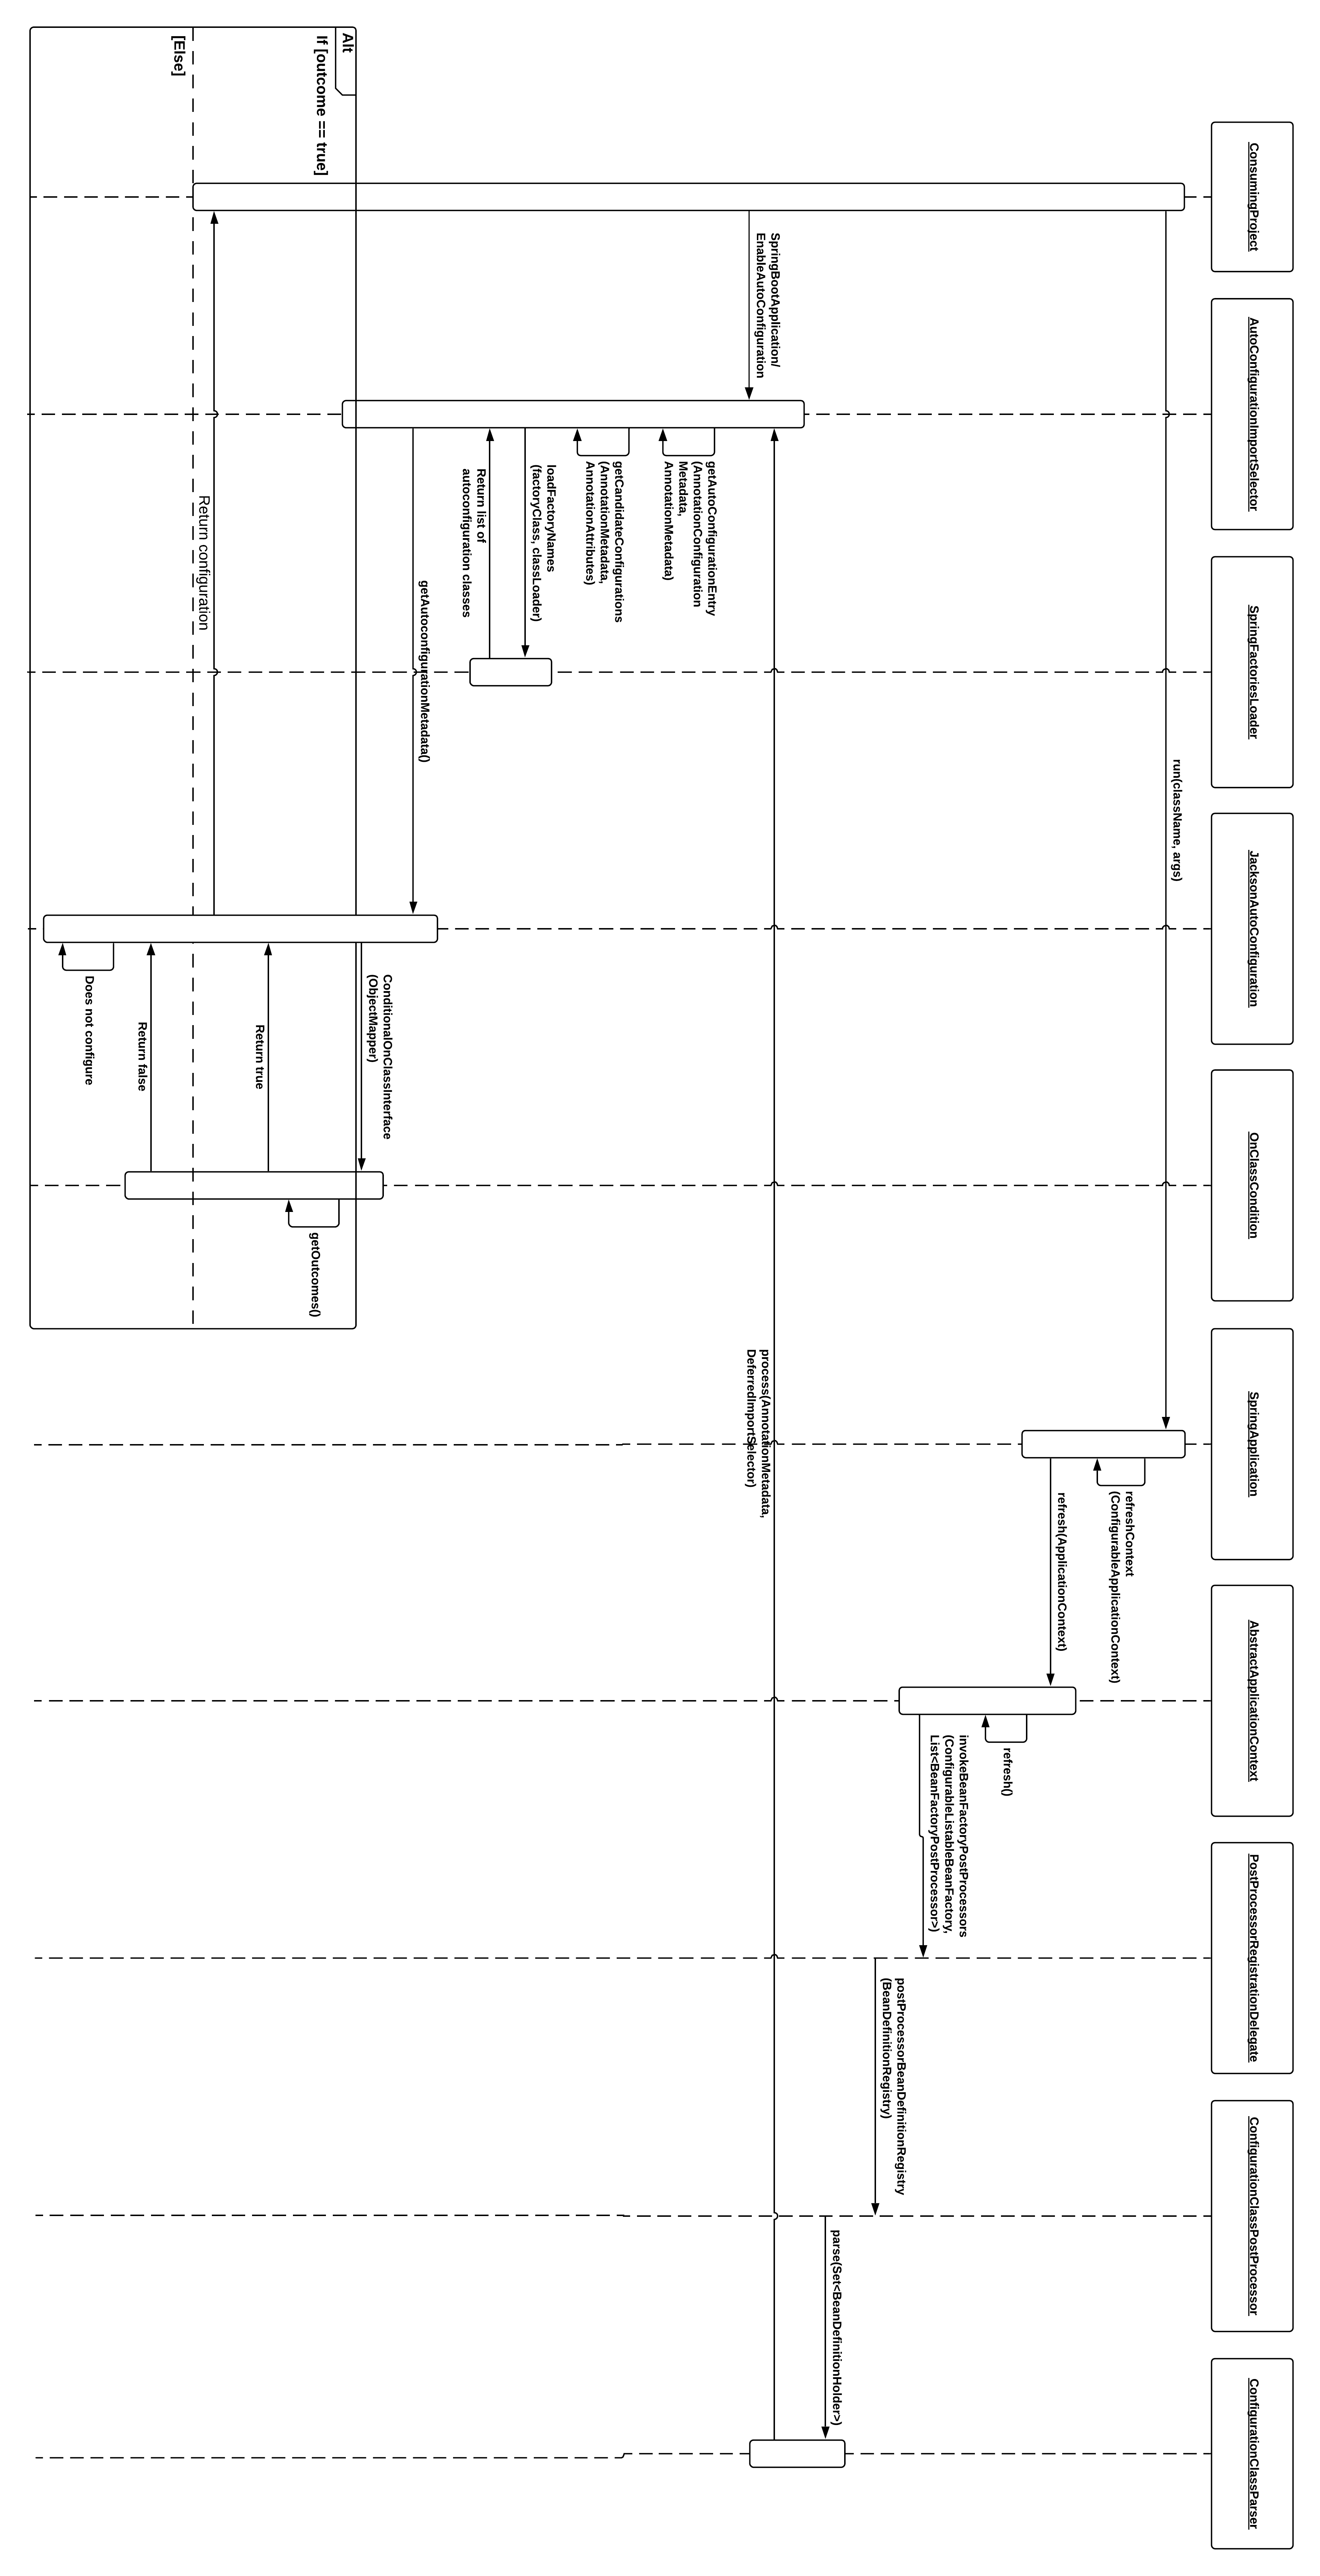
\includegraphics[width=\textwidth, height=.85\textheight, keepaspectratio]{content/architectural-views-top-level/auto-configuration.png}
    \caption{Spring Boot Auto-Configuration Based on Classpath Dependencies}
    \label{sequence-diagram-auto-configuration}
\end{figure}

\textbf{Figure~\ref{sequence-diagram-auto-configuration}}: Consuming projects that use Spring Boot's \texttt{@SpringBootApplication} or \texttt{@EnableAutoConfiguration} will be able to auto-configure their application's dependencies. The figure shows that we are auto-configuring \texttt{Jackson} -- which is a serializer and deserializer library -- in which the \texttt{JacksonAutoConfiguration} class will apply configurations of the \texttt{Jackson} dependency declared in the classpath. The consuming project will use the \texttt{SpringApplication}'s \texttt{run()} method which refreshes the \texttt{ApplicationContext} and eventually invokes the \texttt{AutoConfigurationImportSelector.process()} method. This method will iterate over the pre-defined list of auto-configuration classes defined in the \texttt{spring.factories} file. For each auto-configuration class, the \texttt{AutoConfigurationImportSelector} class will invoke the \texttt{getAutoConfigurationMetadata()} method to call auto-configuration classes to decipher whether or not to configure the consuming project's dependencies. In this particular instance, the called \texttt{JacksonAutoConfiguration} class uses the interface \texttt{@ConditionalOnClass(ObjectMapper.class)} which checks that the \texttt{ObjectMapper} dependency exists in the classpath. If it does, then the \texttt{JacksonAutoConfiguration} class will return the configurations accordingly.

\begin{figure}[H]
    \centering
    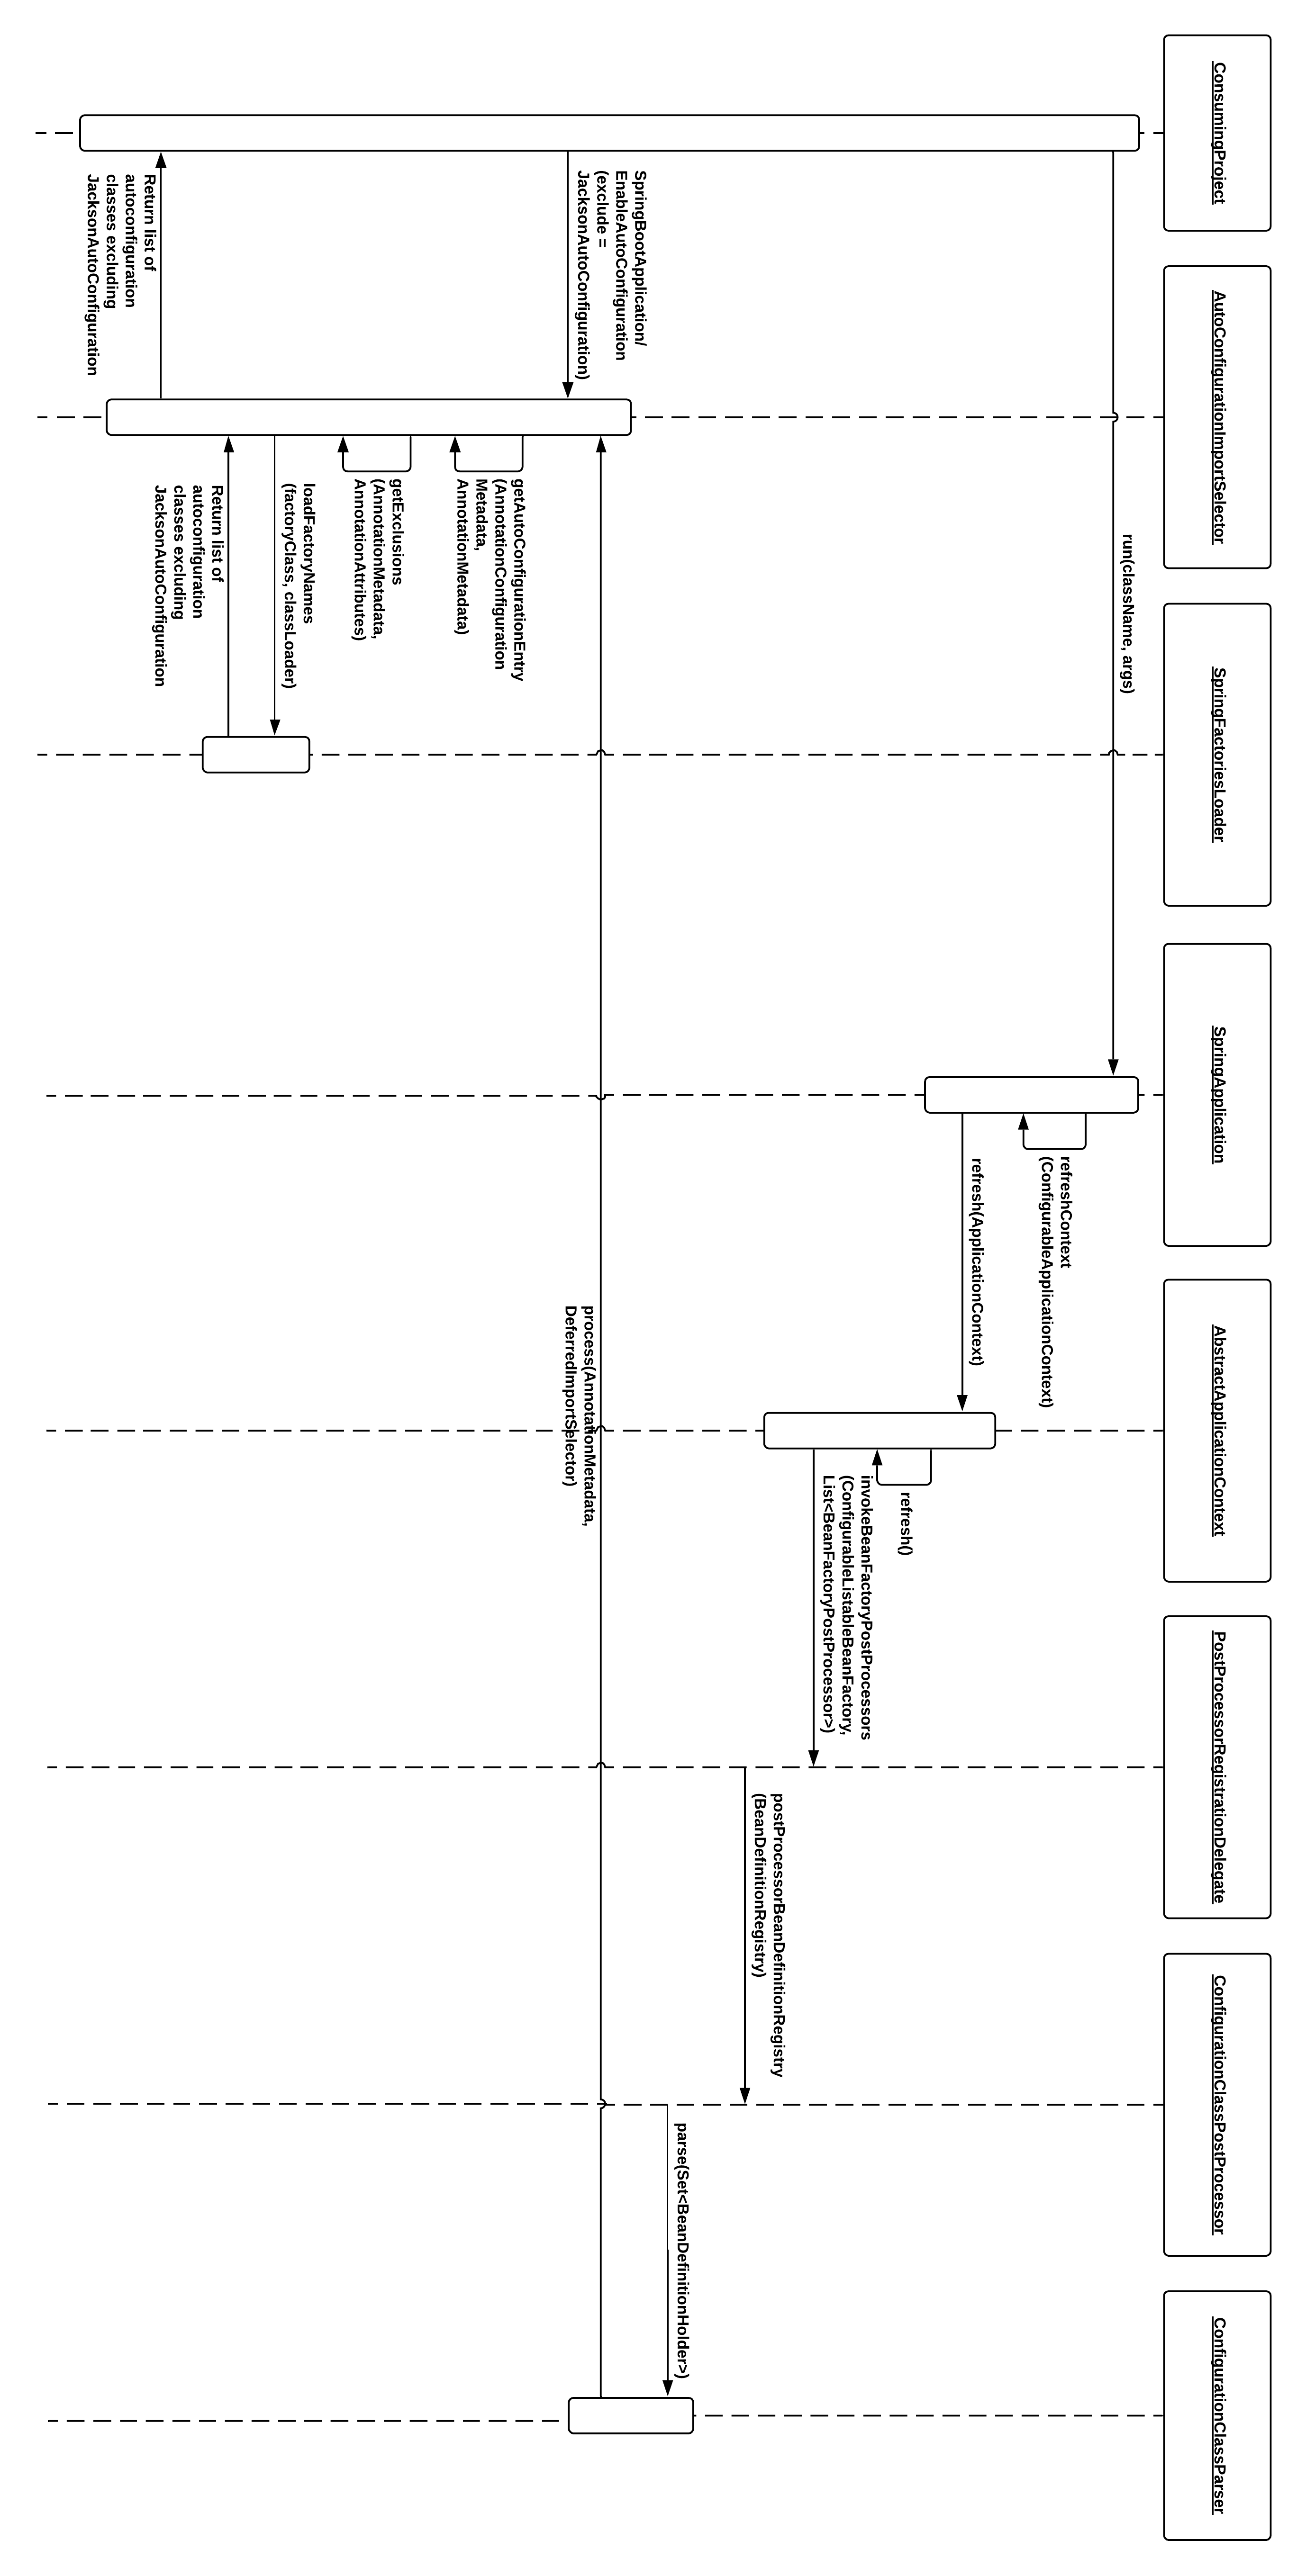
\includegraphics[width=\textwidth, height=\textheight, keepaspectratio]{content/architectural-views-top-level/auto-configuration-exclude.png}
    \caption{Spring Boot Auto-Configuration Exclusion}
    \label{sequence-diagram-auto-configuration-exclude}
\end{figure}

\textbf{Figure~\ref{sequence-diagram-auto-configuration-exclude}}: Consuming projects that use Spring Boot's \texttt{@SpringBootApplication(exclude = JacksonAutoConfiguration.class)} or \texttt{@EnableAutoConfiguration(exclude = JacksonAutoConfiguration.class)} will intently not auto-configure their application's dependency mentioned in the exclude value. The figure shows that we are not auto-configuring \texttt{Jackson}. The consuming project will use the \texttt{SpringApplication}'s \texttt{run()} method which refreshes the \texttt{ApplicationContext} and eventually invokes the \texttt{AutoConfigurationImportSelector.process()} method. This method will iterate over the pre-defined list of auto-configuration classes defined in the \texttt{spring.factories} file excluding the \texttt{JacksonAutoConfiguration} class.

\begin{figure}[H]
    \centering
    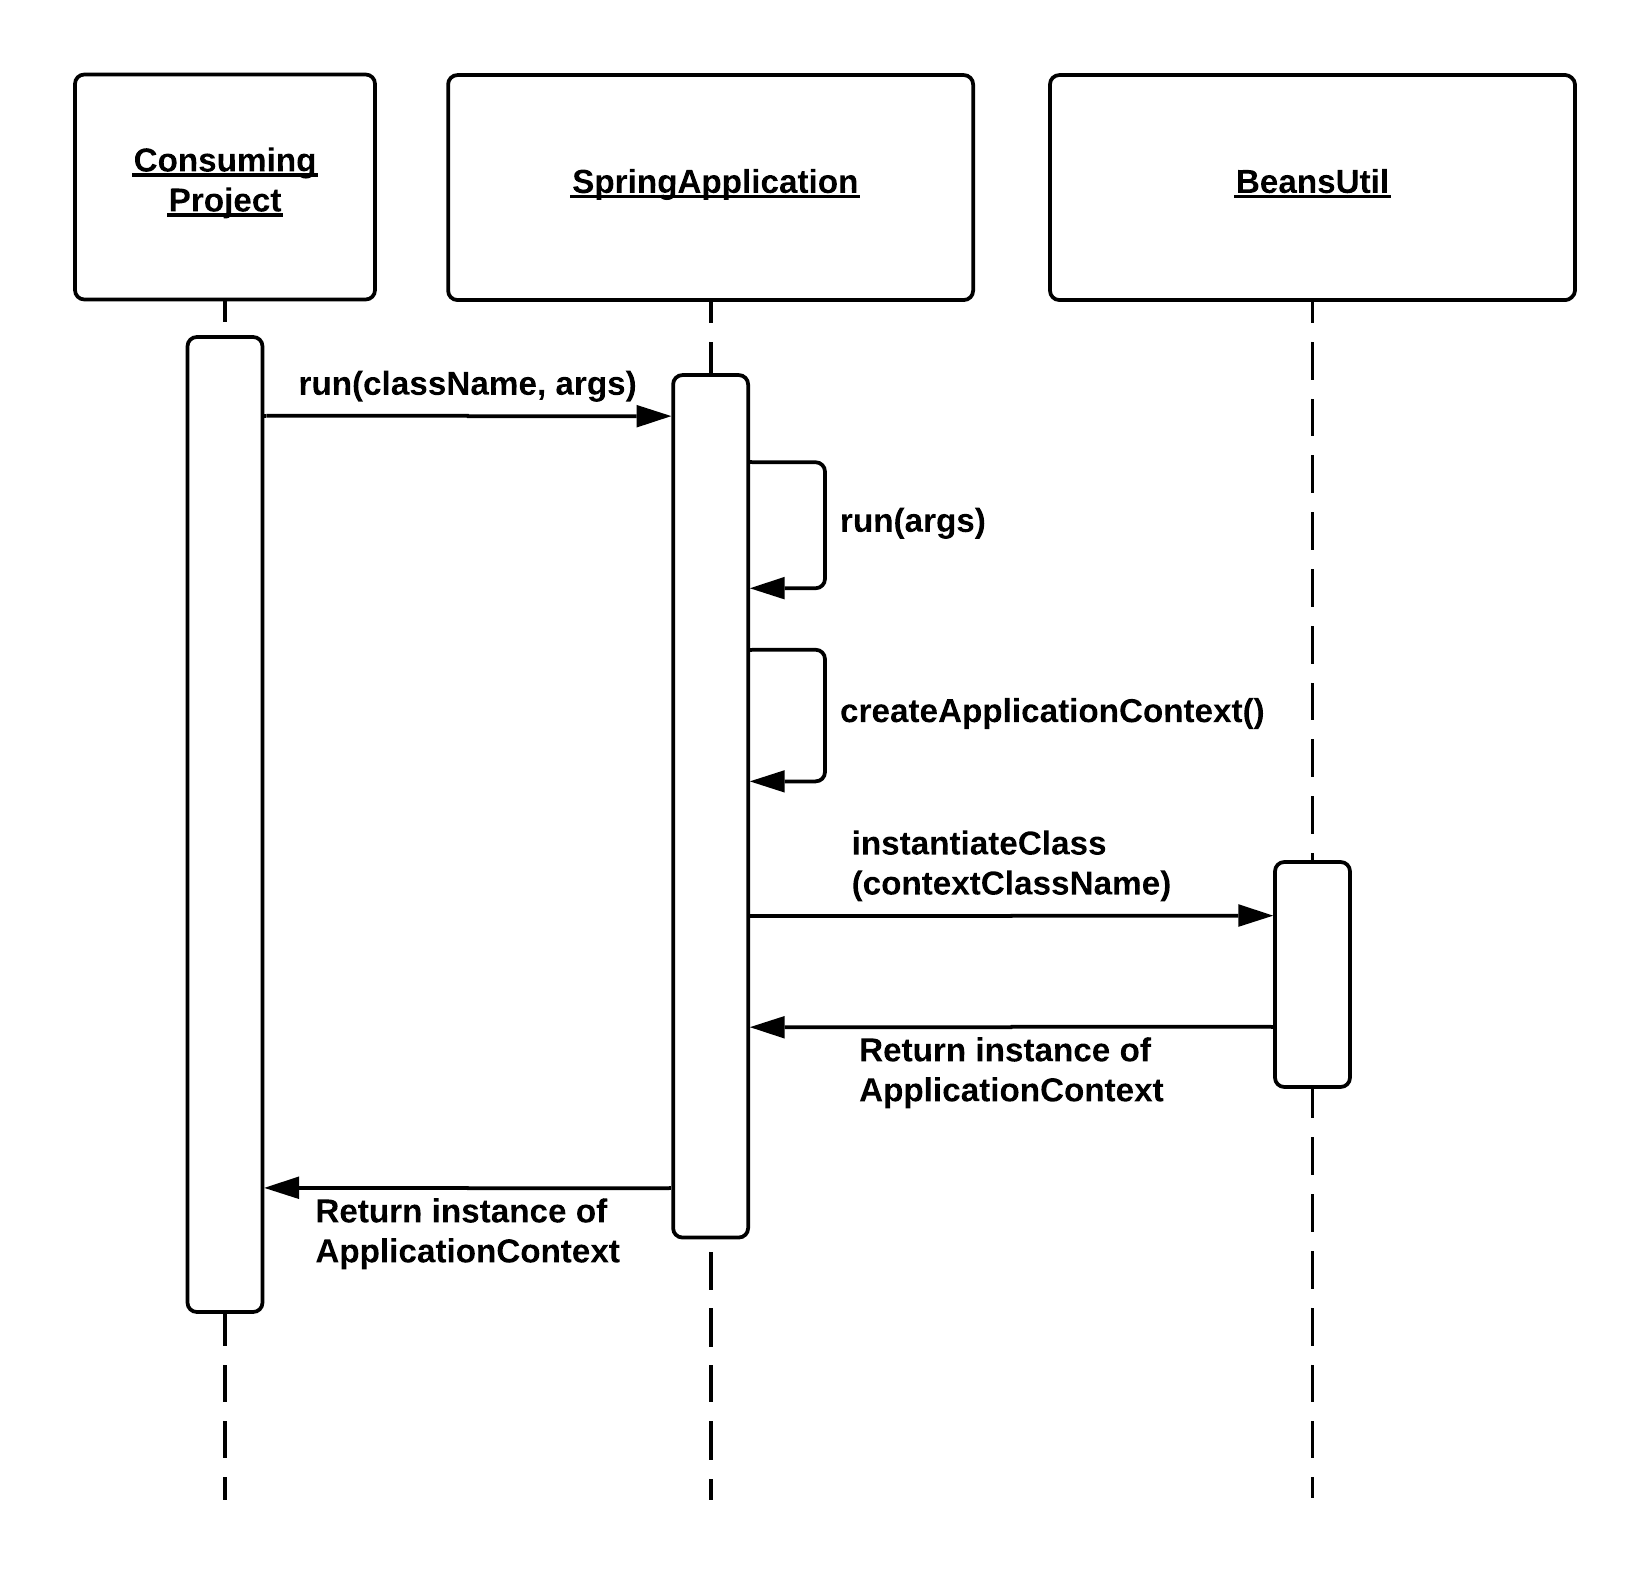
\includegraphics[width=.7\textwidth, height=\textheight, keepaspectratio]{content/architectural-views-top-level/application-context.png}
    \caption{Spring Boot ApplicationContext Creation}
    \label{sequence-diagram-application-context}
\end{figure}

\textbf{Figure~\ref{sequence-diagram-application-context}}: The consuming project will invoke the \texttt{SpringApplication} class' \texttt{run()} method which will self-invoke another overloaded \texttt(run()) method. In this particular \texttt{run()} method, it eventually invokes the \texttt{createApplicationContext()} method that utilizes the strategy pattern to determine the web application type to resolve the context class name. \texttt{SpringApplication} then invokes the \texttt{instantiateClass(contextClassName)} method that returns an \texttt{ApplicationContext} object to the consuming project.

\begin{figure}[H]
    \centering
    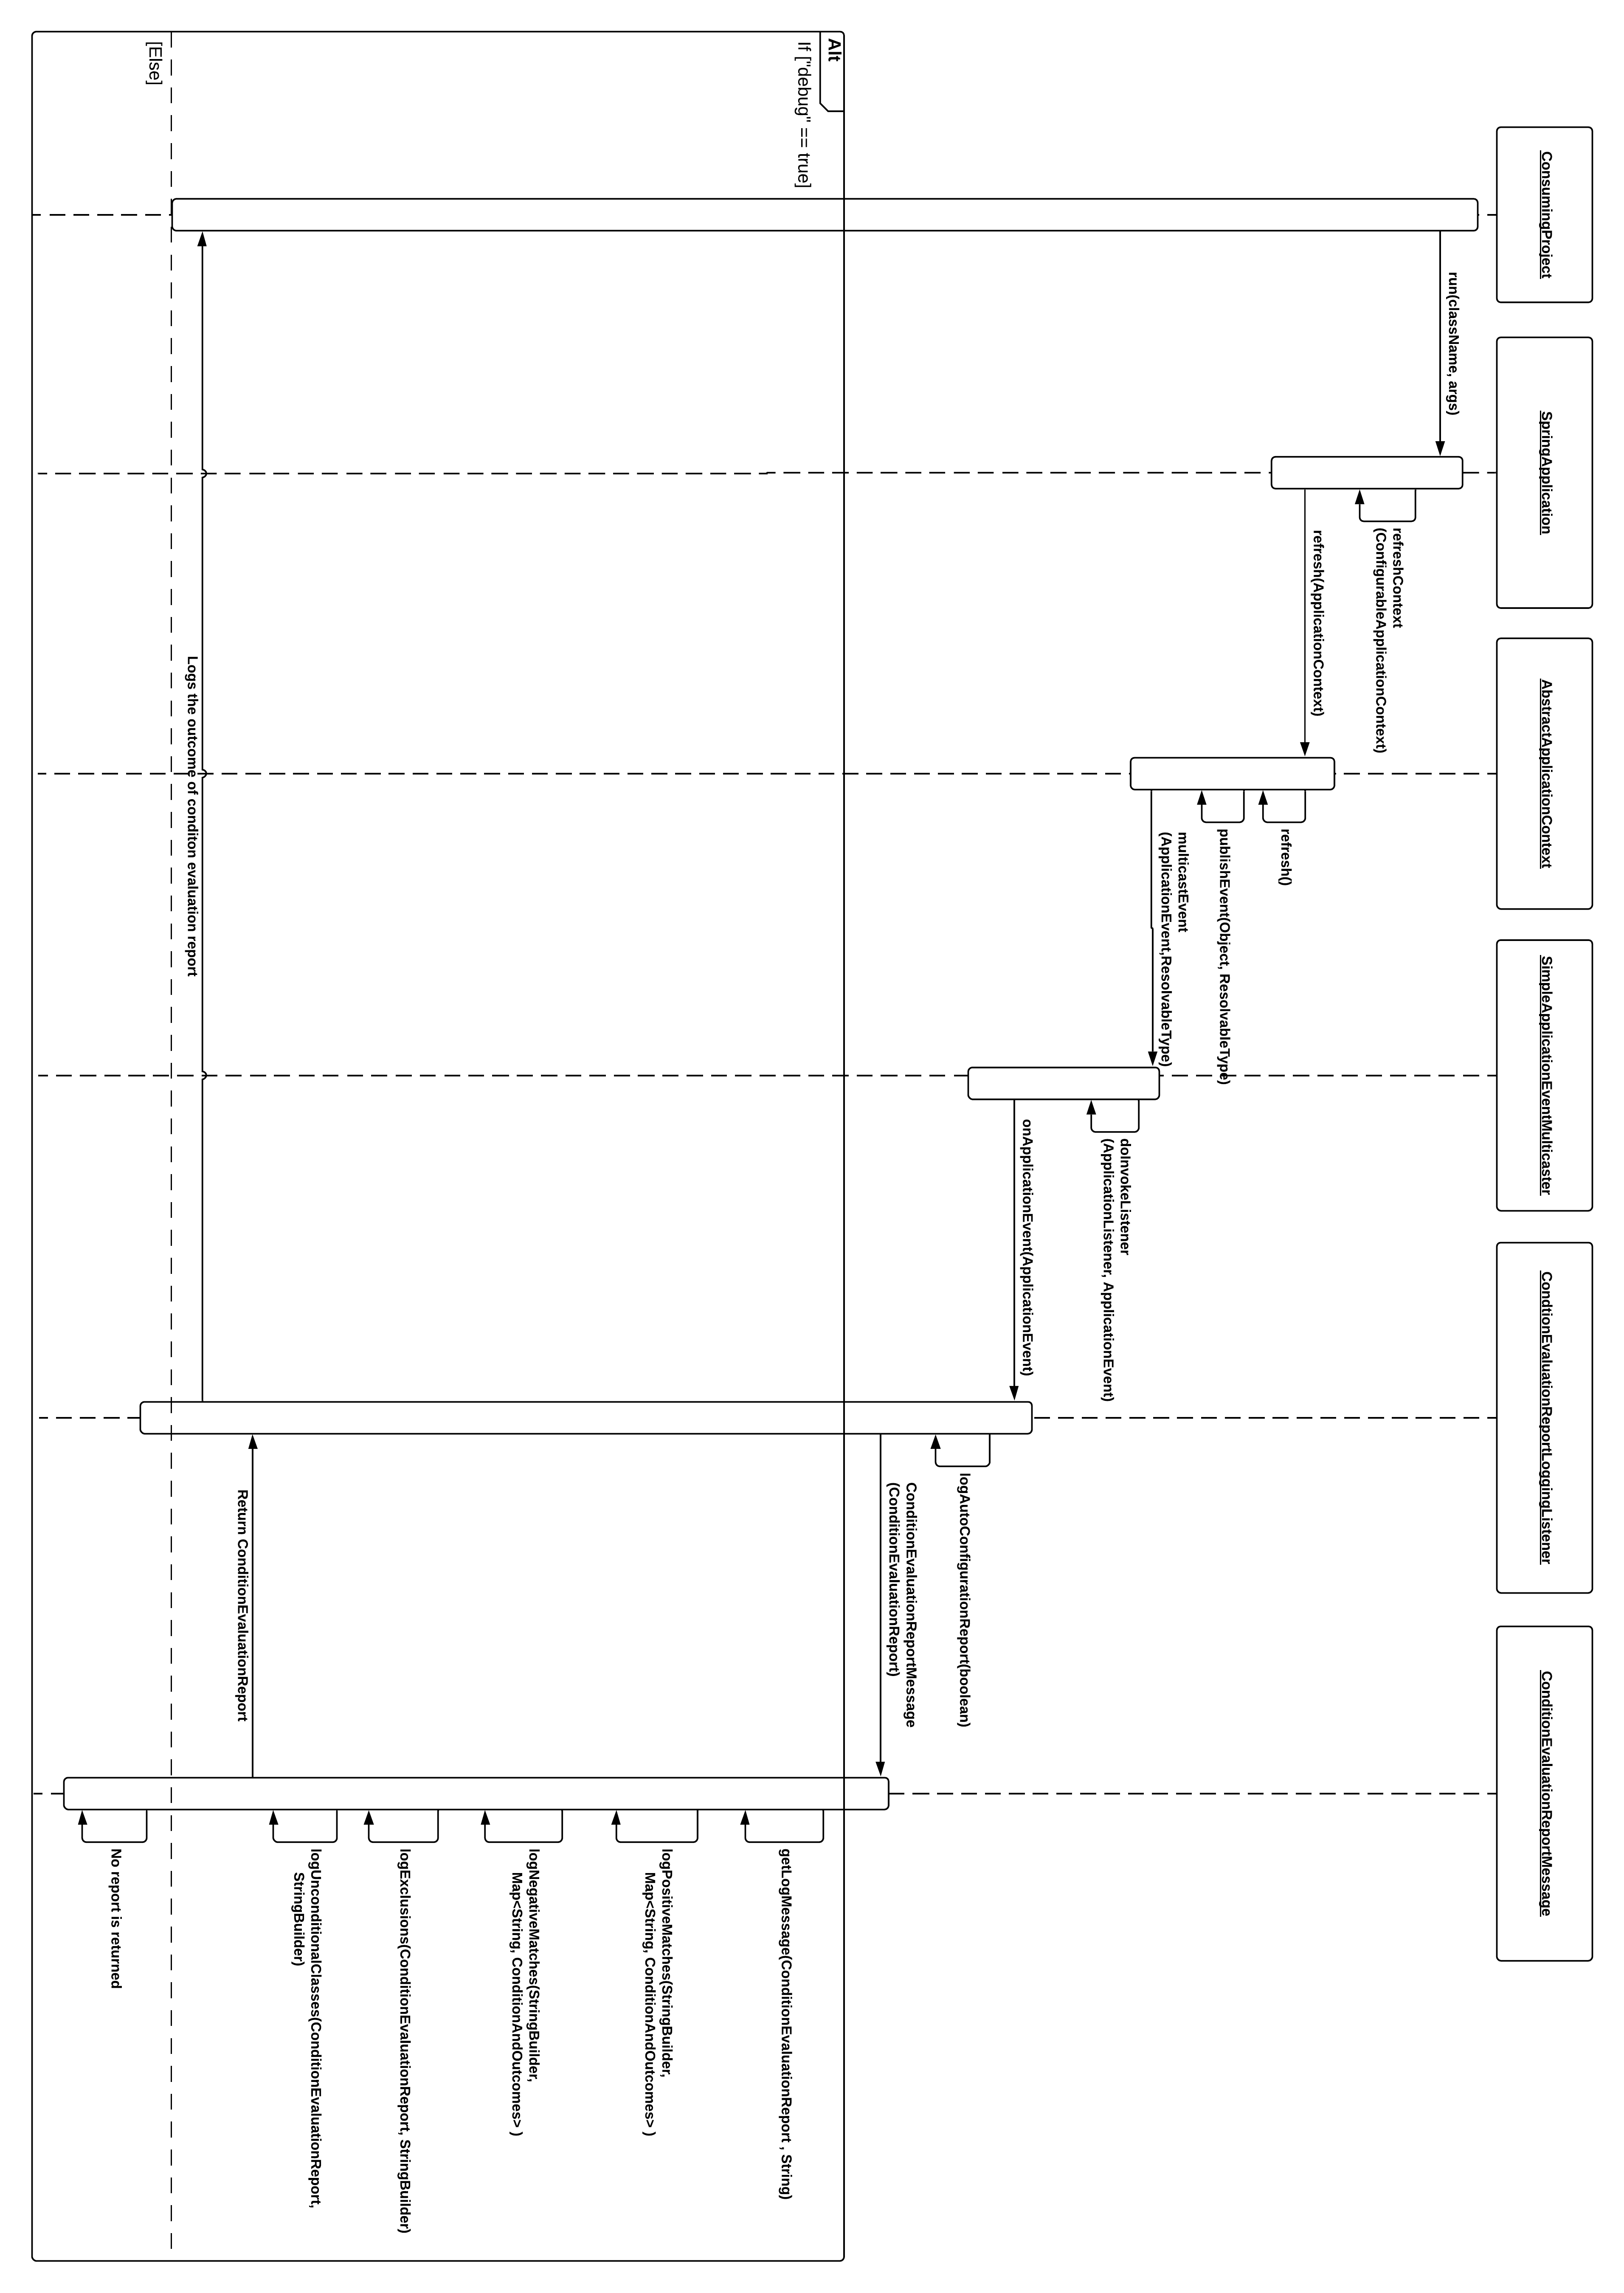
\includegraphics[width=\textwidth, height=\textheight, keepaspectratio]{content/architectural-views-top-level/condition-evaluation-report.png}
    \caption{Spring Boot Condition Evaluation Report}
    \label{sequence-diagram-condition-evaluation-report}
\end{figure}

\textbf{Figure~\ref{sequence-diagram-condition-evaluation-report}}: The consuming project will invoke the \texttt{SpringApplication} class' \texttt{run()} method. Eventually, the \texttt{SimpleApplicationEventMulticaster} class will be invoked by the \texttt{multicastEvent()} method which has an \texttt{ApplicationEvent} argument passed in. The \texttt{SimpleApplicationEventMulticaster} class self-invoke the \texttt{doInvokeListener()} method that listens for the \texttt{ApplicationEvent} which triggers the \texttt{onApplicationEvent()} method, calling all \texttt{*Listener} classes. In this case, the \texttt{ConditionEvaluationReportLoggingListener} class will invoke the \texttt{ConditionEvaluationReportMessage} constructor with the \texttt{ConditionEvaluationReport} as the argument. The \texttt{ConditionEvaluationReportMessage} class will then find the matching outcomes for auto-configuration classes and pre-defined beans when configuring conditional beans. The end result of this process will return the log output of \texttt{ConditionEvaluationReport} if debug is set to true. Otherwise, it will not return the log.

\begin{figure}[H]
    \centering
    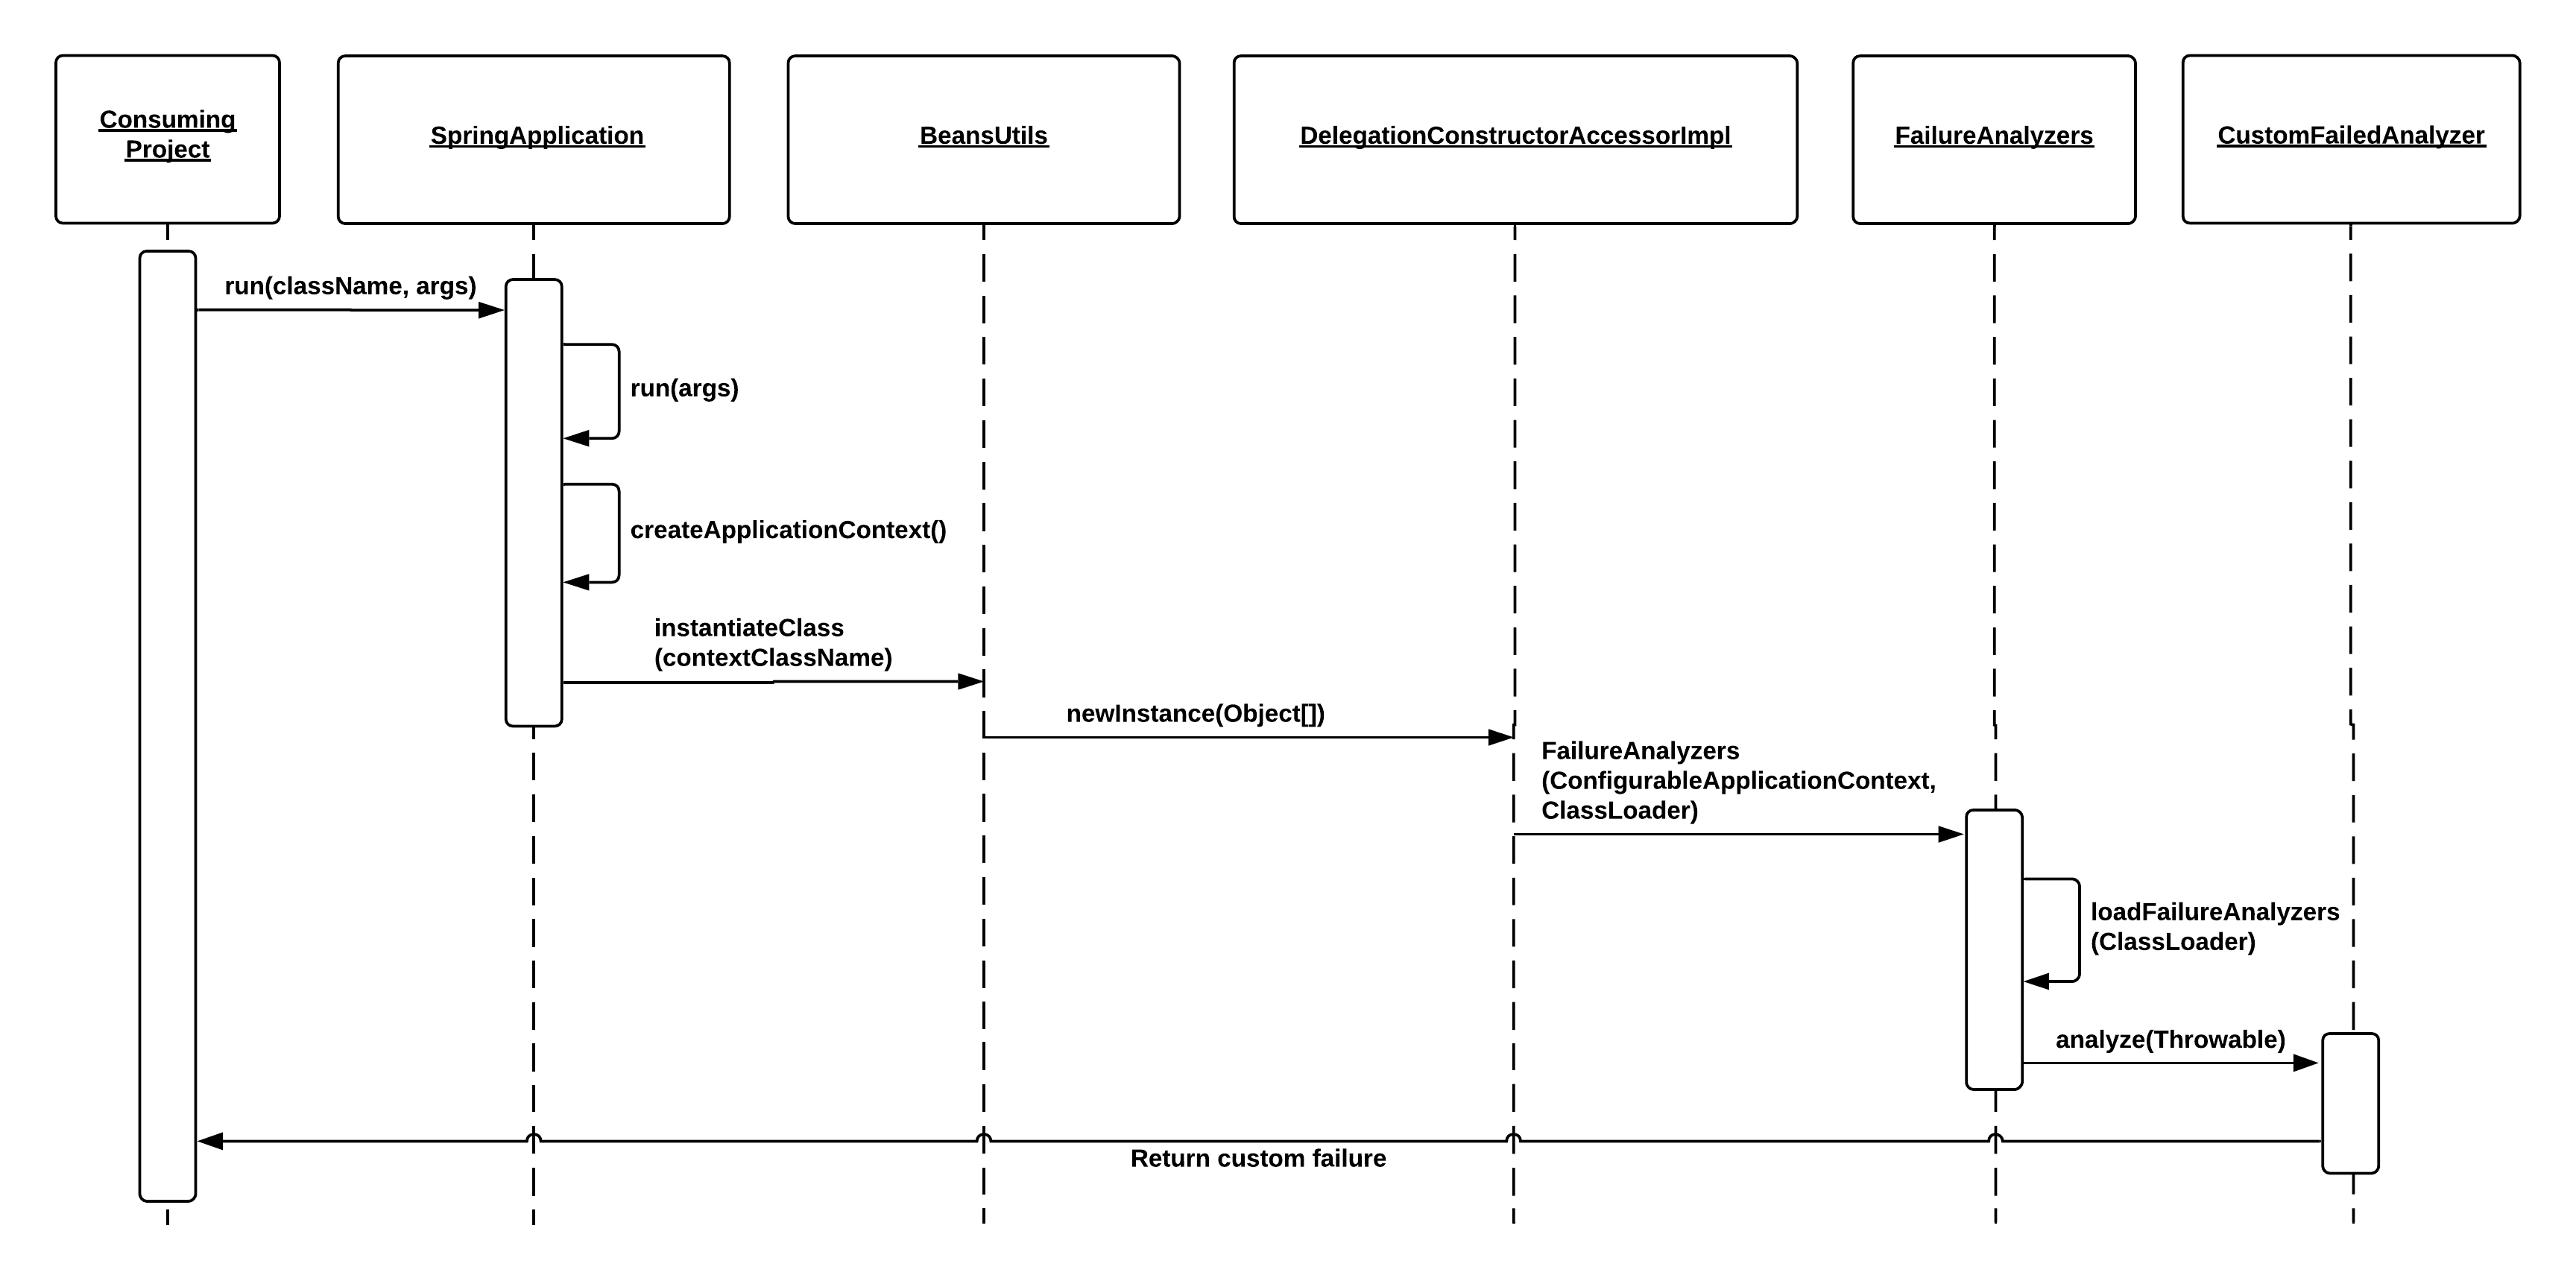
\includegraphics[width=\textwidth, height=\textheight, keepaspectratio]{content/architectural-views-top-level/custom-failure-analyzer.png}
    \caption{Spring Boot Custom Failure Analyzer}
    \label{sequence-diagram-custom-failure-analyzer}
\end{figure}

\textbf{Figure~\ref{sequence-diagram-custom-failure-analyzer}}: The consuming project will invoke the \texttt{SpringApplication} class' \texttt{run()} method and eventually the \texttt{instantiateClass()} method of the \texttt{BeanUtils} class will be invoked. The \texttt{BeanUtils} class will invoke the \texttt{newInstance()} method of the \texttt{DelegationConstructorAccessorImpl} class. This class will invoke the constructor of \texttt{FailureAnalyzers} in which the \texttt{FailureAnalyzers} class will iterate through the list of failure analyzer classes defined in the \texttt{spring.factories} file. In this figure, \texttt{CustomFailedAnalyzer} is a user-defined class which overrides the \texttt{analyze()} method of \texttt{FailureAnalyzers} class. The overridden method of \texttt{analyze()} will return the custom failure as defined in the \texttt{CustomFailedAnalyzer} class.

\section{Information View}

\begin{figure}[H]
    \centering
    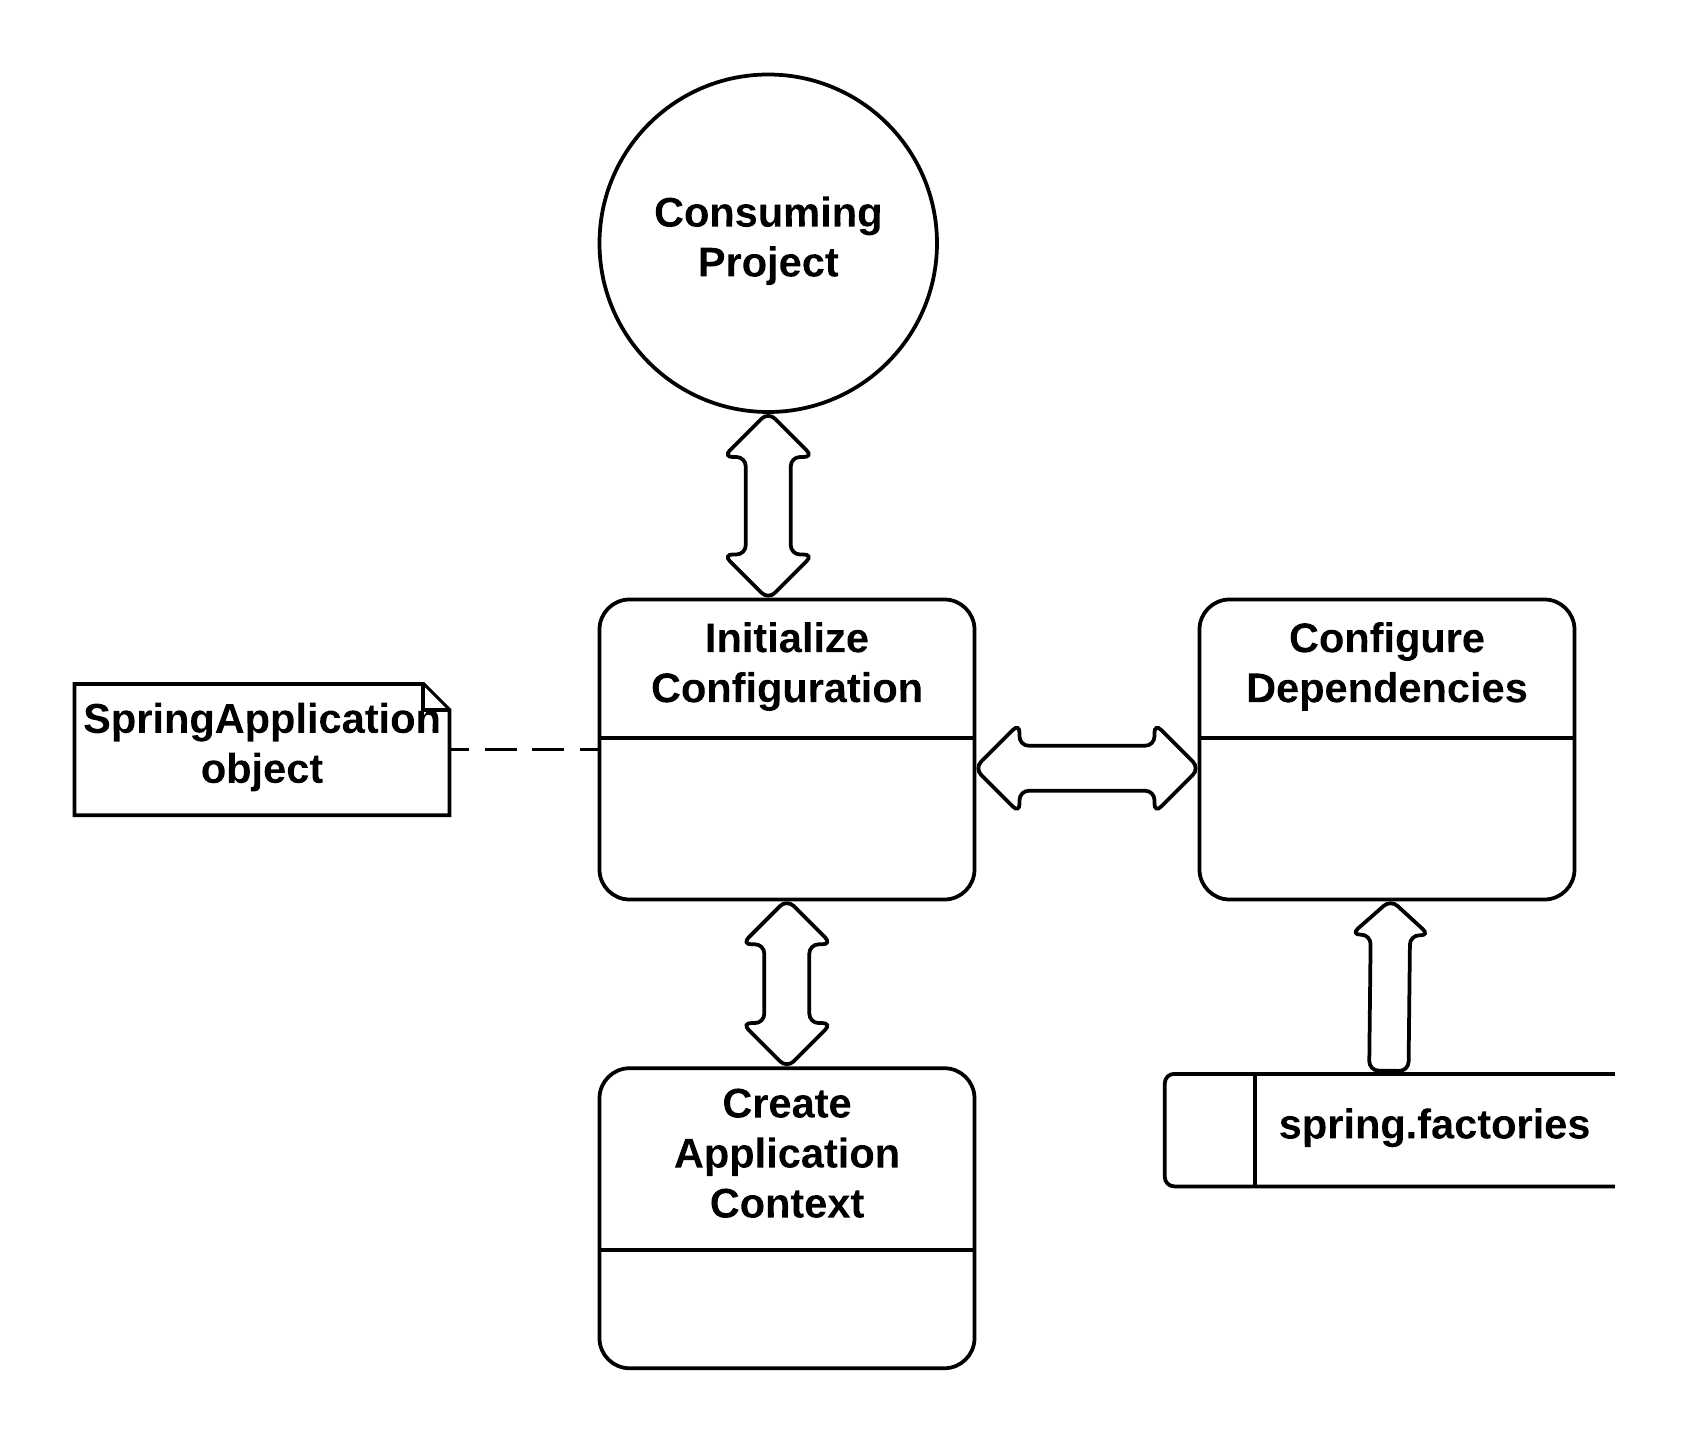
\includegraphics[width=.75\textwidth]{content/architectural-views-top-level/information-flow.png}
    \caption{Spring Boot Configuration Information Flow}
    \label{information-flow-diagram}
\end{figure}

Figure~\ref{information-flow-diagram} shows how data flows throughout a consuming project to auto-configure dependencies. The information flow can be described as the following:

\begin{enumerate}
\item The consuming project as the external entity provides dependencies from its' classpath to the \texttt{SpringApplication} object which initializes the configuration process.
\item The web application type is determined by the classpath dependencies -- of which those dependencies are loaded from the \texttt{ClassLoader} -- which then is passed around to create the application context.
\item Once the application context is created, it will be refreshed to configure dependencies based on the pre-defined list of auto-configuration classes.
\item During the auto-configuration in the configure dependencies process, the list is read from the spring.factories and matched against the loaded classpath dependencies and auto-configure them into beans.
\item Once all of the necessary beans are created, the application context will again refresh to load in all of the beans and return to the \texttt{SpringApplication} object which passes the application context to the consuming project.
\end{enumerate}

\begin{figure}[H]
    \centering
    \includegraphics[width=.7\textwidth]{content/architectural-views-top-level/information-lifecycle.png}
    \caption{Spring Boot Configuration Information Lifecycle}
    \label{information-lifecycle-diagram}
\end{figure}

Figure~\ref{information-lifecycle-diagram} shows the Spring Boot auto-configuration lifecycle, which is simple from a high level view. Once the application context is created, and then the application context is refreshed to configure dependencies. Once those dependencies are configured, the application context again is refreshed and the lifecycle ends.\\

\subsection{Data Quality}

\textbf{Timeliness and Latency}: The Spring Boot module and the data on which it manipulates is essentially static data after its' runtime processes are finished. Spring Boot will be able to use the new data as soon as the application is restarted. Consider the following scenario:

\begin{quote}
\textit{The consuming project has third-party dependencies used in a dependency management tool. When the consuming project starts up and the Spring Boot module is able to use the dependencies to help configure dependencies. While the application is up and running, the user decides to make changes in the dependency management tool, however, the changes are not reflected during this time.}
\end{quote}

The consuming project has to be restarted in this situation to reflect the changes made in dependency management tool. These changes will also be reflected in the configuration that Spring Boot behind the scene.\\

\textbf{Archiving and Information Retention}: Archiving and information retention is not important in Spring Boot module as it depends on the consuming project to provide the data for configuration. It is up to the consuming project on how they manage the data and then Spring Boot can then leverage that to help in configuration.\\

\textbf{Information Quality}: As the consuming project modifies the dependencies in the dependency management tool, the information in terms of configuration will not be reflected unless the consuming project is started up or restarted. In terms of information quality, we would say it is moderate as it updates the configuration on the next application start-up but not in real-time.

\section{Deployment View}

Spring Boot is a software framework first and foremost, and it therefore requires a mechanism to be deployed as an artifact for consumption. In this particular case, Spring Boot relies on Maven Central as it's main distribution artifact repository. Users are able to pull down the Spring Boot artifact from Maven Central to use the provided interfaces and functionalities that it offers for Java web application development.

The mechanism by which Spring Boot is deployed is done through their automated server called \texttt{Concourse}. However, the means to get it running in Concourse is not automated. According to the Spring Boot documentation for their continuous integration pipeline, a specific command is issued through the command line to trigger the pipeline. The following is the command to do the aforementioned:\\

\begin{lstlisting}[language=bash, caption={Start Continuous Integration Pipeline Command \cite{springbootconcourse:online}}]
$ fly -t spring-boot set-pipeline -p spring-boot-2.3.x -c ci/pipeline.yml -l ci/parameters.yml
\end{lstlisting}\ \\

In the above command, the file \texttt{ci/pipeline.yml} is a set of instructions to be run from top to bottom. The \texttt{ci/parameters.yml} provides the \texttt{ci/pipeline.yml} file a set of arguments to be passed in through interpolation. On a high level, the pipeline.yml file calls other \texttt{*.yml} files which have their own instructions. These files can be found in the \texttt{ci/tasks} directory and include the following \cite{springboottasks:online}:

\begin{itemize}
\item \textbf{build-deployment-tests.yml}: File that calls the \texttt{ci/scripts/build-deployment-tests.sh} script which initially calls another script called \texttt{common.sh}. The \texttt{common.sh} script will create a soft link between the current working directory's \texttt{embedmongo} file to the home directory and then cleans the local repository of old dependencies. This process will go back to the \texttt{build-deployment-tests.sh} script and run the deployment tests with the embedded \texttt{MongoDB} managed process against a local \texttt{distribution-repository} file.
\item \textbf{build-integration-tests.yml}: File that calls the \texttt{ci/scripts/build-integration-tests.sh} script which initially calls another script called \texttt{common.sh}. The \texttt{common.sh} script will create a softlink between the current working directory's \texttt{embedmongo} file to the home directory and then cleans the local repository of old dependencies. This process will go back to the \texttt{build-integration-tests.sh} script and run the integration tests with the embedded \texttt{MongoDB} managed process against a local \texttt{distribution-repository} file.
\item \textbf{build-project.yml}: File that calls the \texttt{ci/scripts/build-project.sh} script. The script checks the results of the integration tests that were ran to verify that the results meet a specified acceptance criteria, and if it does, then it will proceed to deploy the Spring Boot framework release to the Artifactory repository.
\item \textbf{build-smoke-tests.yml}: File that calls the \texttt{ci/scripts/build-smoke-tests.sh} script which initially calls another script called \texttt{common.sh}. The \texttt{common.sh} script will create a softlink between the current working directory's \texttt{embedmongo} file to the home directory and then cleans the local repository of old dependencies. This process will go back to the \texttt{build-smoke-tests.sh} script and run the smoke tests with the embedded \texttt{MongoDB} managed process against a local \texttt{distribution-repository} file.
\item \textbf{detect-jdk-updates.yml}: File that calls the \texttt{ci/scripts/detect-jdk-updates.sh} script. The script checks that each of their self-managed Docker images of OpenJDK 8, 11, and 13 are up to date with the latest releases. This is done by making a network GET request to\\ \texttt{https://api.adoptopenjdk.net/v2/info/releases/openjdk8} and extracting information from the response. Based on this extraction, the script can determine If there is a need to upgrade any of the aforementioned OpenJDK versions. If there is, then the script will dynamically create an issue on the Spring Boot GitHub repository through a network POST request with the extracted information from the response.
\item \textbf{generate-release-notes.yml}: File that calls the \texttt{ci/scripts/generate-release-notes.sh} script. The script will invoke jar file called \texttt{github-release-notes-generator.jar} with provided arguments that contain GitHub credentials as well as path to the Spring Boot GitHub repository. The end result is a produced file called \texttt{release-notes.md} that is directly put into GitHub. It will also version and tag the release.
\item \textbf{promote.yml}: File that calls the \texttt{ci/scripts/promote.sh} script. The script will define an environment variable called \texttt{BUILD\_INFO\_LOCATION}. The environment variable's value gives a path to a json file called \texttt{build-info.json} on the local machine, which in itself contains information about their Artifactory repository. Using the environment variable, the \texttt{promote.sh} script promotes and distributes through the various stages which has an associated release type, namely: milestone, release candidate, and release. After this, the script publishes the Spring Boot artifact as a plugin.
\item \textbf{stage.yml}: File that calls the \texttt{ci/scripts/stage.sh} script. The script will locally pull down a copy of the Spring Boot project from GitHub and deploy it to a Artifactory repository based on the release type. Then, it will run all smoke, integration, and deployment tests against that deployed artifact.
\item \textbf{sync-to-maven-central.yml}: File that calls the \texttt{ci/scripts/sync-to-maven-central.sh} script. The script will synchronize the release artifact in Artifactory repository to the Maven Central repository.
\end{itemize}

Each of the files have their own purpose and concern, and are called at different times of the pipeline but it is important to remember that it is ultimately the \texttt{pipeline.yml} that orchestrates all of the above functionalities of the automated pipeline. Figure ~\ref{deployment-diagram} shows the relationship between the runtime components during the automated pipeline process:

\begin{figure}[H]
    \centering
    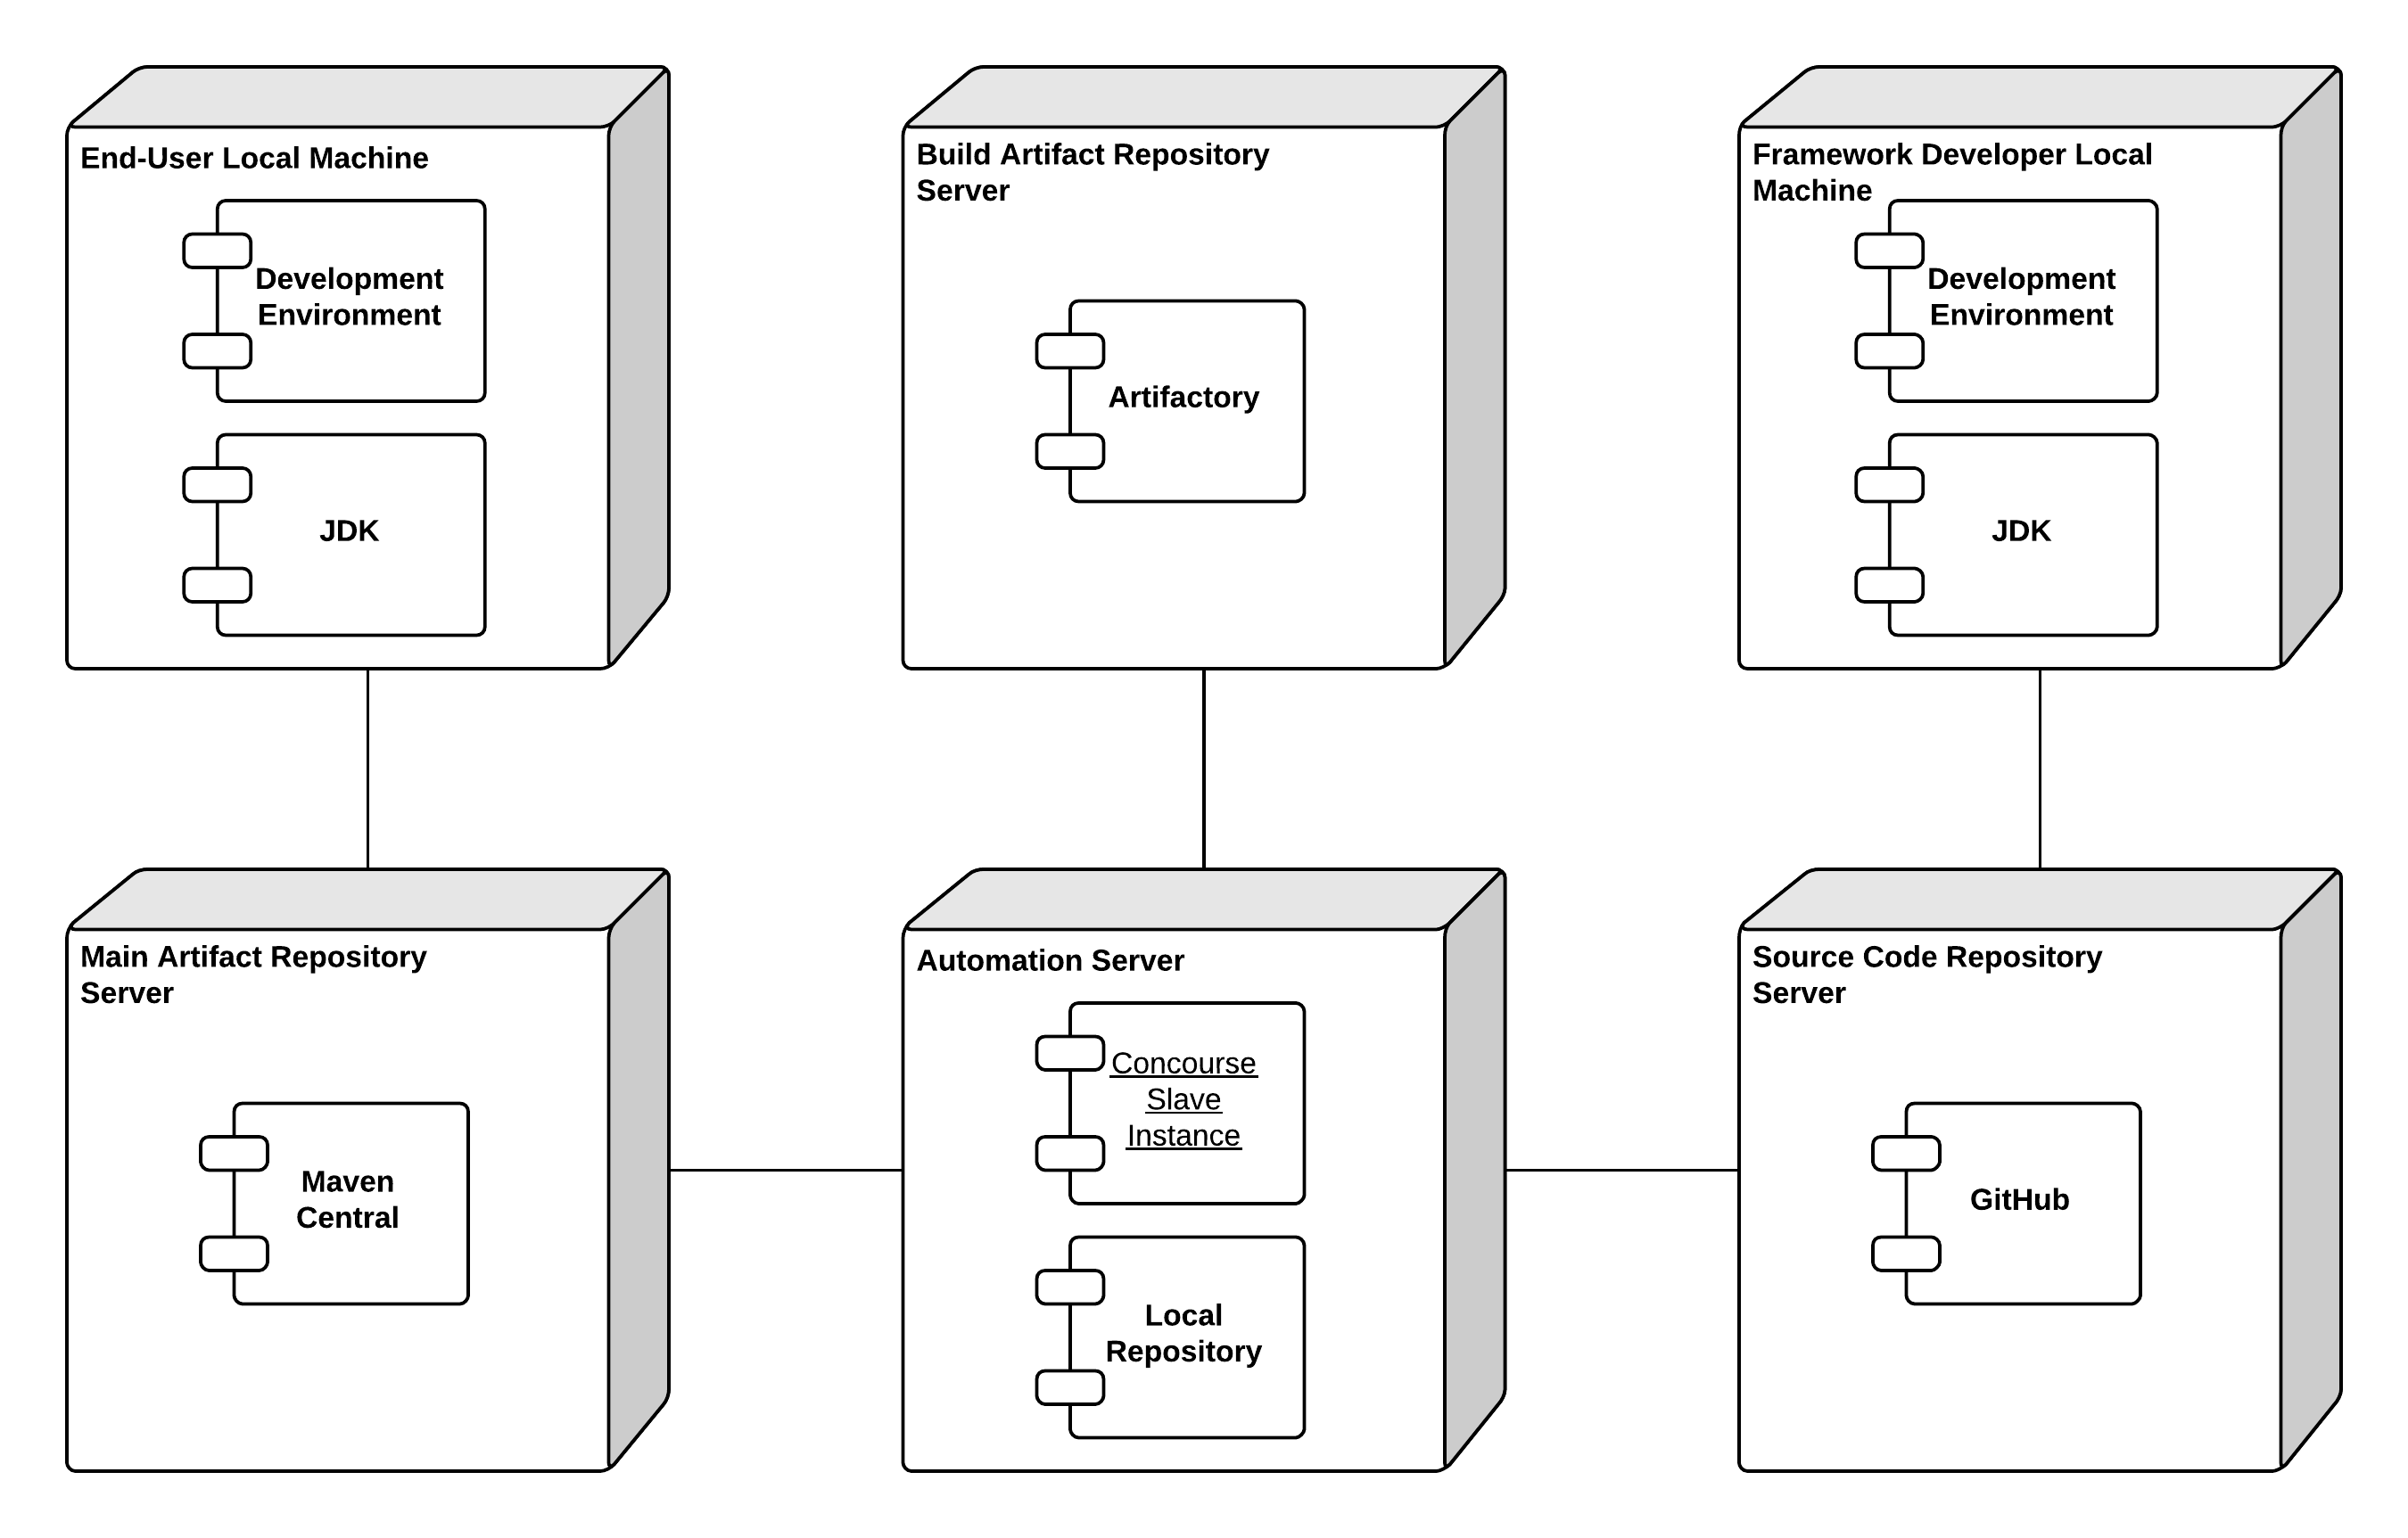
\includegraphics[width=\textwidth]{content/architectural-views-top-level/deployment-diagram.png}
    \caption{Spring Boot Deployment Diagram}
    \label{deployment-diagram}
\end{figure}

The goal of this automated pipeline process is to give releases of the Spring Boot framework to end-users. End-users in this context, being Java developers who want to create web applications quickly. They can integrate the Spring Boot framework into their projects by sourcing it from the Maven Central repository and declaring it as a dependency in their dependency management tool. The following dependency definition below shows generically how it can be sourced and declared:\\

\clearpage

\begin{lstlisting}[caption=Representation of Dependency Management for Spring Boot]

plugins {
	id 'java'
    id 'org.springframework.boot' version '2.2.1.RELEASE'
	id 'io.spring.dependency-management'
}

repositories {
    mavenCentral()
}

dependencies {
    implementation 'org.springframework.boot:spring-boot-starter-web'
    implementation 'org.springframework.boot:spring-boot-starter-data-mongodb'
}
\end{lstlisting}\ \\

This is the final step to get the Spring Boot framework in the hands of Java developers to build their web application.

\chapter{Appendices}
\section{Proposed Changes}

In the latest release version 2.2.1, the Spring Boot team described in their release notes a feature that optionally allows a user to globally lazy initialize pre-defined beans to increase the performance of the start-up time \cite{springBootReleaseNote}. The idea is to initialize pre-defined beans only at the time of usage and not during start-up. According to the Spring Boot release notes, there are a few downsides that need to be considered when using the feature:

\begin{itemize}
\item "Handling of HTTP requests may take longer while any deferred initialization occurs" \cite{springBootReleaseNote}.
\item "Failures that would normally occur at start-up will now not occur until later" \cite{springBootReleaseNote}.
\end{itemize}

On every first HTTP request after start-up, the pre-defined beans needed to make the request will be initialized and will be kept in the application context until the web application is restarted or shutoff. Delaying the pre-defined beans until this point is still an expense that needs to be paid, so the first HTTP request will also be slower than subsequent identical requests. Though in the greater picture, this is a very low cost to pay for a faster start-up. The issue with the feature really boils down to potential bean initialization errors that can show up during the first HTTP request, which may not be an ideal situation depending on the consuming project's testing strategy. As the release notes said, it will normally occur during start-up, but not with the global lazy initialization feature enabled. To partially mitigate this potential issue of the feature, an \texttt{@lazy(false)} annotation can be used on pre-defined beans that are understood to common amongst all available HTTP requests. The disadvantage of the annotation is that users have to identify and maintain those common pre-defined beans. These are trade-offs that have to be considered.\\

Spring Boot is by design, a means to reducing development time and effort; going straight to the point of developing business logic that matters. To keep the same mentality, we believe that although the \texttt{@lazy} annotation may be created with good intentions, we would like to propose a new way to control lazy initialization in the same way but without having the need to declare the \texttt{@lazy} annotation on any specific bean.\\

Assuming the global lazy initialization feature is enabled and the web application is started up for the first time after, we can use an algorithm to monitor pre-defined bean usages and based off of that, cache all most commonly used pre-defined bean's information into a file at the root directory level of the consuming project. The idea here being that on a restart after this point, the beans defined in the cache file will be auto-configured along side all dependencies in the classpath that have auto-configuration classes as listed in the \texttt{spring.factories} file. If a pre-defined bean has been removed from the codebase before the restart, then the cache file will update to reflect based on the list of classpath dependencies gathered by the \texttt{AutoConfigurationImportSelector} class. The algorithm will also be smart enough to add and remove pre-defined beans based on usage on next start-up.\\

Not all users will want to use this proposed feature, but we feel that can be a very beneficial choice to be given an option to use. The way this proposed feature will be declared is by using a new annotation named \texttt{@EnableAutoLazyInitialization} in the consumer project's application class, with the pre-requisite being that @SpringBootApplication or @EnableAutoConfiguration is also declared in same class. The @EnableAutoLazyInitialization would be implemented by a new class AutoBeanImportSelector which would handle the logic to update the cache with the most commonly used beans and it would also need the help of AutoConfigurationImportSelector to check on if the classpath dependencies have been changed.\\

We may need to have further consideration into the design on how the proposed extension will connect with the existing architecture. Figure ~\ref{extension-diagram} below diagrams our proposal:

\begin{figure}[H]
    \centering
    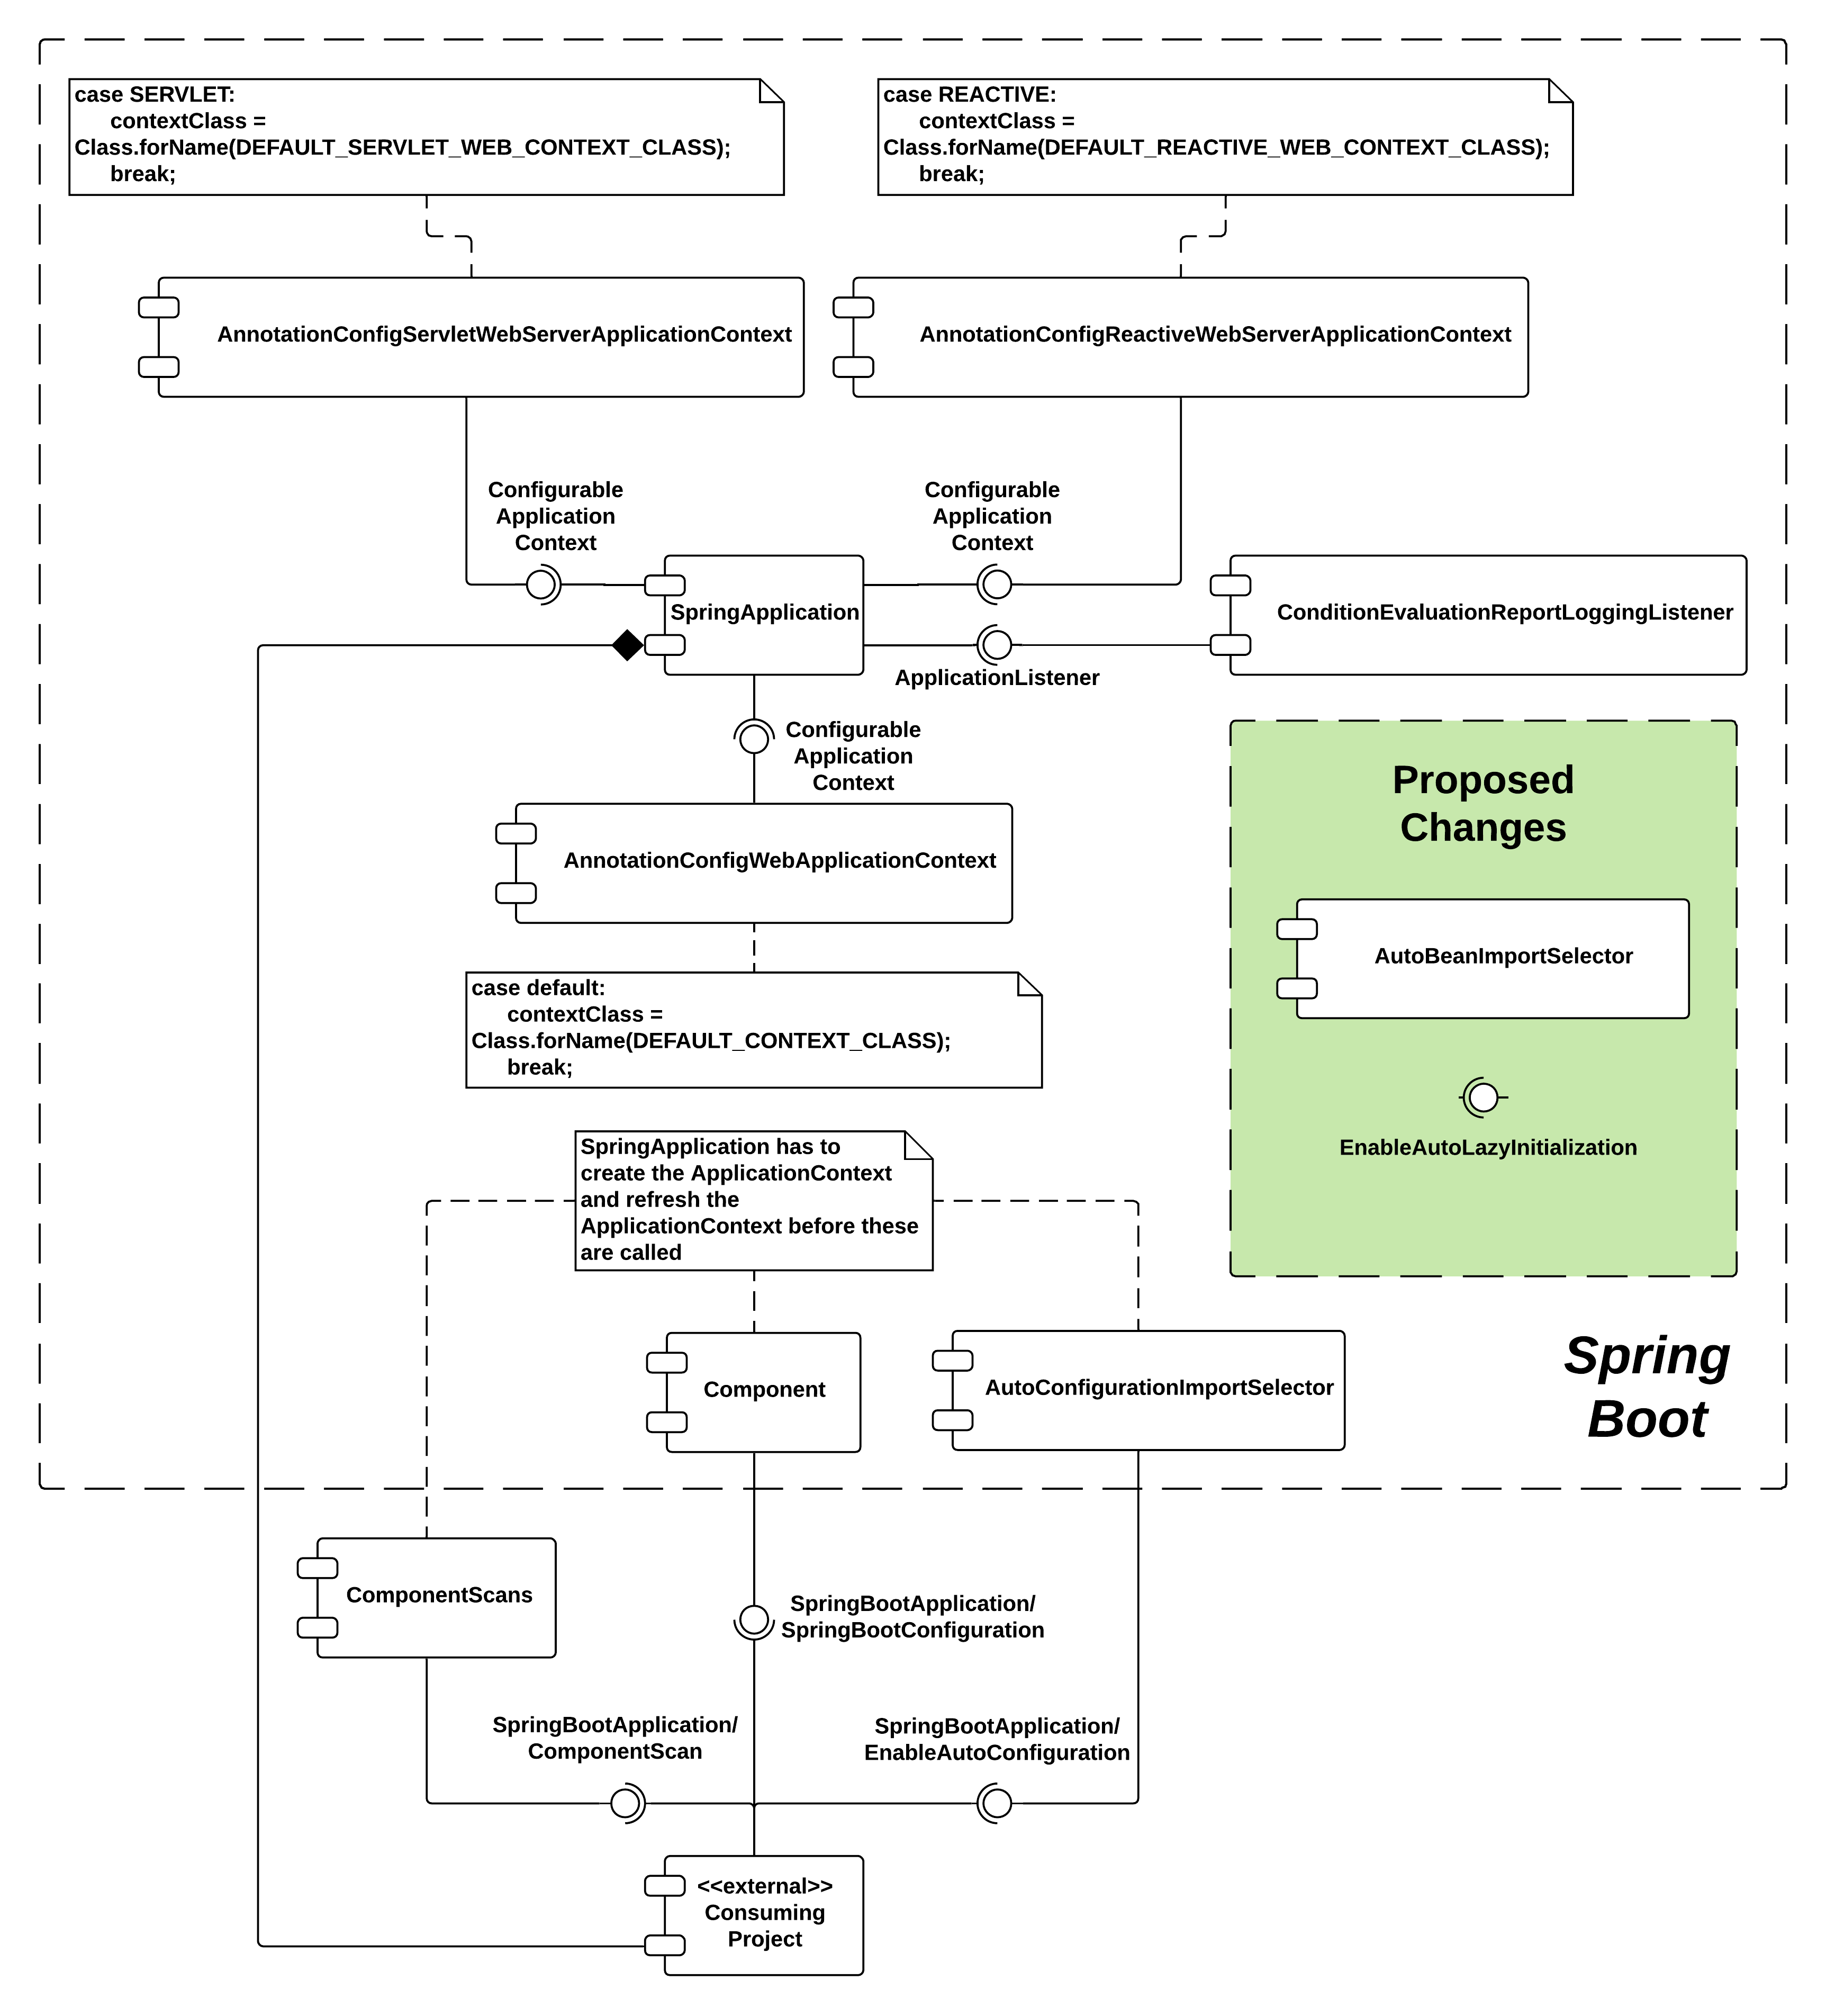
\includegraphics[width=\textwidth]{content/appendices/extension.png}
    \caption{Spring Boot Extension Proposal Diagram}
    \label{extension-diagram}
\end{figure}


\bibliographystyle{content/appendices/ieee-annot}
\bibliography{content/appendices/phase-3}

\end{document}
